\documentclass[10pt, compress]{beamer}

\usetheme{m}

\usepackage{booktabs}
\usepackage[scale=2]{ccicons}
\usepackage{minted}
\usepackage{wrapfig}
\usepackage{enumitem}% http://ctan.org/pkg/enumitem
\usepackage[font=scriptsize,labelfont=bf]{caption}
\usepackage{natbib}

\def\bibfont{\footnotesize}

\usepgfplotslibrary{dateplot}

\usemintedstyle{trac}

\title{Estimation of Terrain Gradient Conditions \& Obstacle Detection Using a Monocular Vision-based System}
\subtitle{Final Demonstration}
\date{\today}
\author{Connor Luke Goddard (clg11)}
\institute{Department of Computer Science, Aberystwyth University}

\begin{document}

\maketitle

\plain{Background}

\begin{frame}[fragile]
  \frametitle{Background}
  
  \vspace{-10pt}
	
     \begin{block}{}  

	          \begin{wrapfigure}{r}{0.4\textwidth}
   \vspace{-20pt}
  \begin{center}
    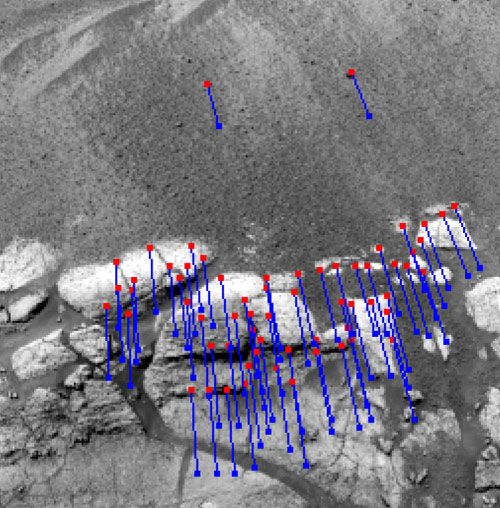
\includegraphics[width=0.25\textwidth]{mars.jpg}
  \end{center}
  \vspace{-15pt}  \caption{Tracked features from MER [2].}
  \end{wrapfigure}
  
  The ability for an autonomous robot to navigate from one location to another in a manner that is both \textbf{safe}, yet \textbf{objective} is vital to the \textbf{survivability} of the machine, and the \textbf{success of the mission} it is undertaking.    
		
       \end{block}

\vspace{15pt}
	
   \begin{block}{}
Vision based obstacle detection has enjoyed a high level of research focus over recent years. Less work has concentrated on providing a means of reliably detecting changes in terrain slope through the exploitation of observed changes in motion. 
  \end{block}


\end{frame}

\begin{frame}[fragile]
  \frametitle{Related Work}
  
  	\begin{enumerate}[label={[\arabic*]}]
  	
  		\item \textbf{\textit{A Robust Visual Odometry and Precipice Detection
System Using Consumer-grade Monocular Vision}}, J. Campbell \textit{et al.}, IEEE, 2005

		\item \textbf{\textit{Obstacle Detection using Optical Flow}}, T. Low and G. Wyeth, School of Information Technology and Electrical Engineering, University of Queensland, 2011
		
		\item \textbf{\textit{Appearance-based Obstacle Detection with Monocular Color Vision}}, I. Ulrich and I. Nourbakhsh, AAAI, 2000
  			
  	\end{enumerate}
  	
  	\vspace{5pt}
  	
  	
  	\begin{figure}[ht!]
\centering
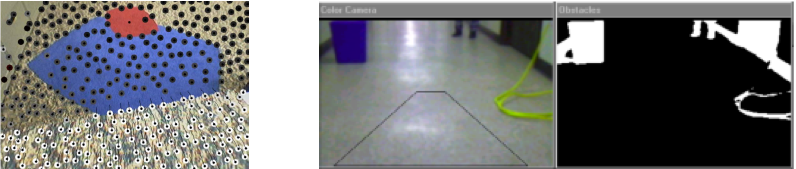
\includegraphics[scale=0.3]{related_work.png}
    \caption{\textbf{Left:} Precipice detection [1], \textbf{Right:} Obstacle colour detection [3]}
  \end{figure}

  	
\end{frame}

\begin{frame}[fragile]
  \frametitle{Project Overview}
  
  \begin{block}{Focus}
    Investigation into a system capable of utilising a single, forward-facing colour camera to provide an estimation into current terrain gradient conditions, obstacle location \& characteristics and robot ego-motion. 
  \end{block}
  
  
  \begin{block}{Potential Metrics For Observation}
   
  \begin{itemize}[label={\textbullet}]
  	\item Changes in terrain gradient (i.e. slopes).
  	\item Location \& characteristics of positive and negative obstacles (i.e. rock or pit respectively).
  	\item Current robot speed of travel.
  	\item Changes in robot orientation.
  \end{itemize}
  
 \end{block}
 
\end{frame}

\plain{Working Hypothesis}

\begin{frame}[fragile]
  \frametitle{Working Hypothesis}

	\hspace*{20pt} \textit{``From images captured using a \textbf{non-calibrated} monocular camera system, analysis of optical flow vectors extracted using \textbf{localised appearance-based} dense optical flow techniques can provide certain estimates into the current condition of terrain gradient, the location and characteristics of obstacles, and robot ego-motion.''}

\end{frame}

\begin{frame}[fragile]
  \frametitle{Motion Parallax}

  Approach focussed on the effects of \textbf{motion parallax}. \\ \vspace{0.5cm}
  
  \textbf{i.e.} Objects/features that are at a greater distance from the camera appear to  move less from frame-to-frame than those that are closer.
  
\begin{figure}[ht!]
\centering
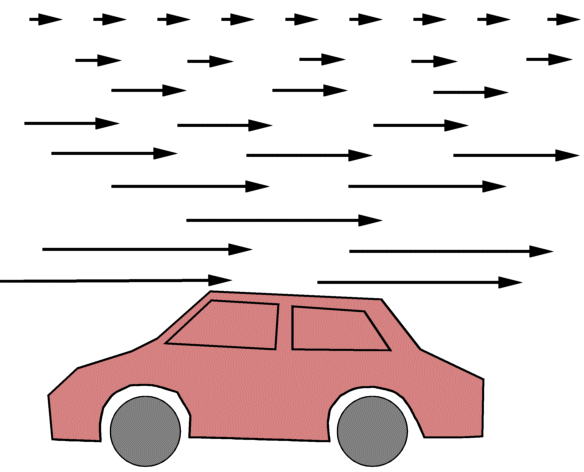
\includegraphics[scale=0.2]{motion_parallax.png}
    \caption{Typical example of motion parallax [4].}
  \end{figure}
  
\end{frame}

\begin{frame}[fragile]
  \frametitle{Inference of Terrain Gradient \& Obstacle Detection}

  \begin{block}{Key Aspects}
   
  \begin{enumerate}[label={\arabic*.}]
  \item The exclusive use of appearance-based template matching techniques to provide a localised variant of dense optical flow analysis over the use of sparse optical flow techniques relying upon a high number of available image features.
  \item The use of a formalised model to represent detected changes in vertical displacement as part of efforts to estimate changes in terrain gradient in addition to the location characteristics of potential obstacles. 
\end{enumerate}
  
 \end{block}
 
\end{frame}

\begin{frame}[fragile]
  \frametitle{Vertical Displacement Model}
  
  \vspace{-35pt}

 Provides a mechanism by which to evaluate the prediction:
 
 \vspace{15pt}
 
       \begin{wrapfigure}{r}{0.5\textwidth}
   \vspace{-30pt}
  \begin{center}
    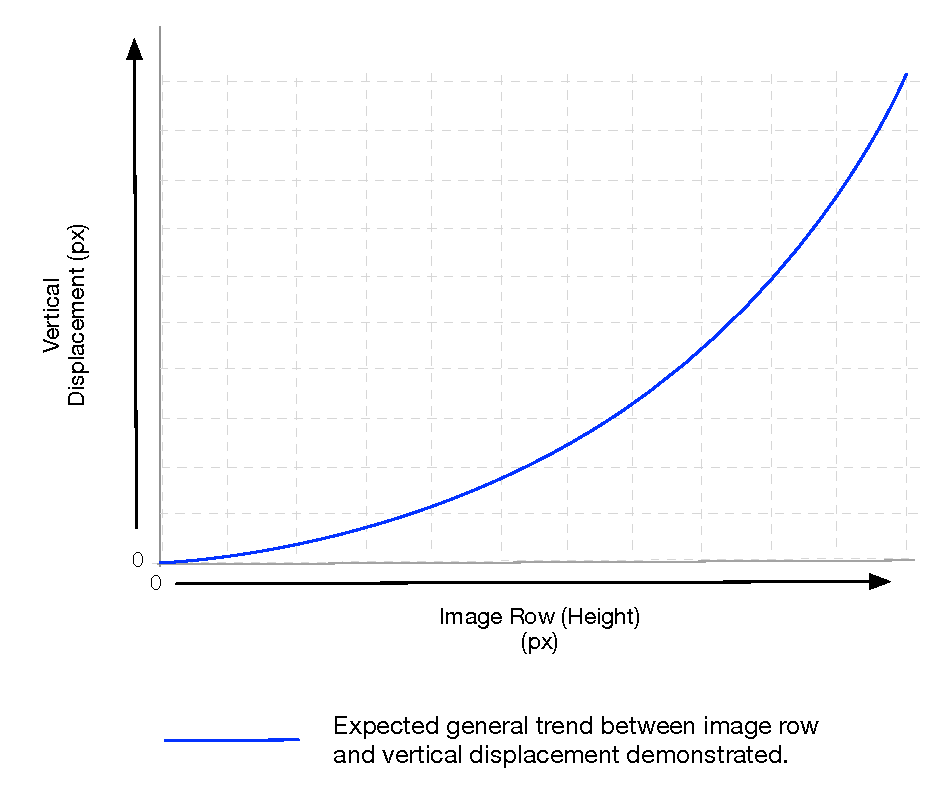
\includegraphics[width=0.52\textwidth]{model.pdf}
  \end{center}
  \vspace{-15pt}
  \caption{Example of ``perfect" vertical displacement model.}
  \end{wrapfigure}
   
%   \hspace*{20pt} 
   
  \textit{``Features captured towards the \textbf{bottom} of an image will show \textbf{greater displacement} between subsequent frames, than those features captured towards the \textbf{top} of the image."}
   
\end{frame}

\begin{frame}[fragile]
  \frametitle{Inference of Terrain Slope \& Potential Obstacles}

From observing discrepancies between the current model and ``baseline" model, it should be possible to infer the presence of potential obstacles: 

  \begin{figure}[ht!]
\centering
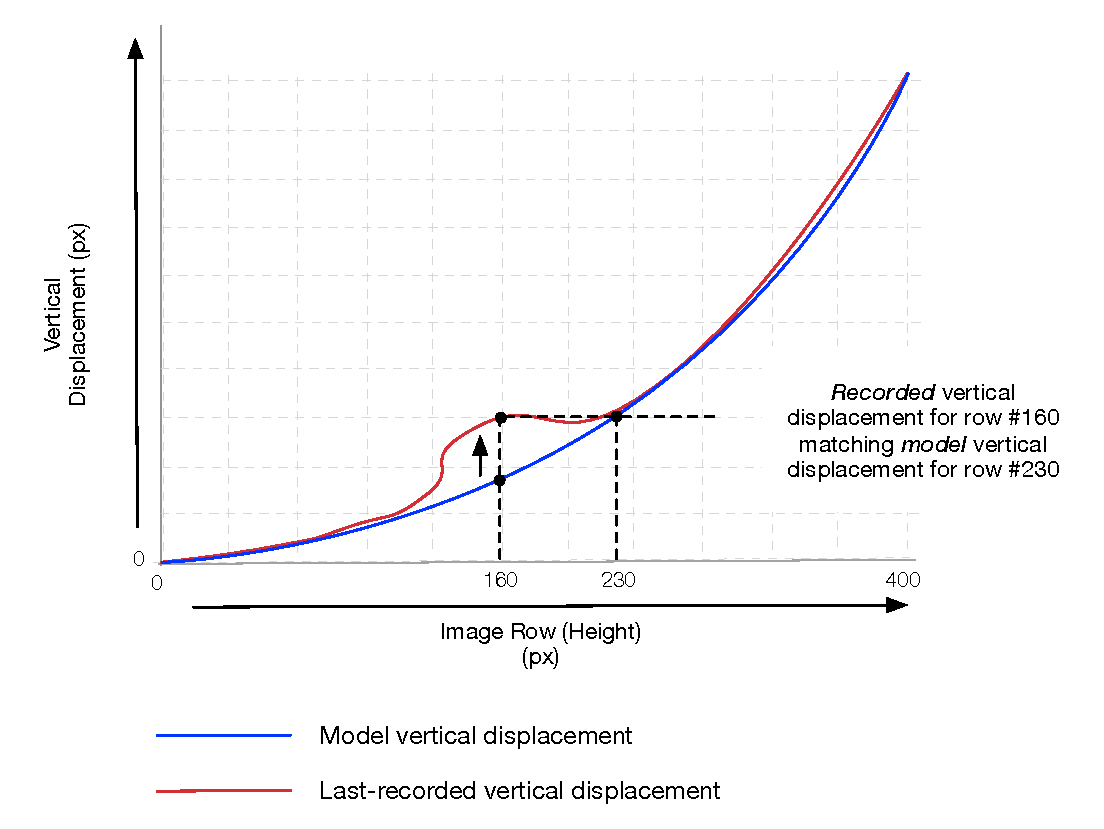
\includegraphics[scale=0.3]{obstacle_graph}
\caption{Vertical displacement model indicating the potential presence of a positive obstacle.}
  \end{figure}
  
  
\end{frame}

\begin{frame}[fragile]
  \frametitle{Inference of Terrain Slope \& Potential Obstacles}

Differences in model discrepancy behaviour should provide enough information to establish between a potential obstacle and a change in terrain slope: 

  \begin{figure}[ht!]
\centering
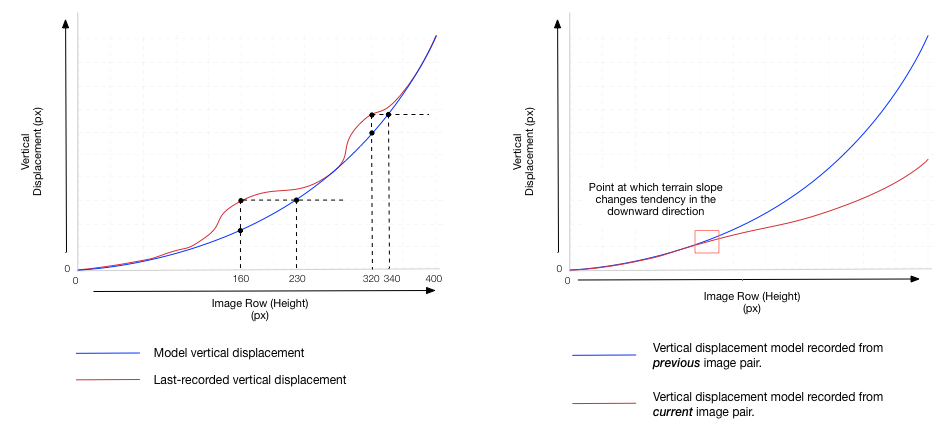
\includegraphics[scale=0.28]{slope_vs_obstacle}
\caption{Example of observed differences between detection of obstacles and change in terrain slope.}
  \end{figure}
  
  
\end{frame}

\begin{frame}[fragile]
  \frametitle{Robot Rotation}
  
\vspace{-10pt}

Two types of observed motion:

\begin{itemize}[label={\textbullet}]
  	\item \textbf{Translation} (\textit{Vertical} component of optical flow vectors)
  	\item \textbf{Rotation} (\textit{Horizontal} component of optical flow vectors)
  \end{itemize}

  \begin{figure}[ht!]
\centering
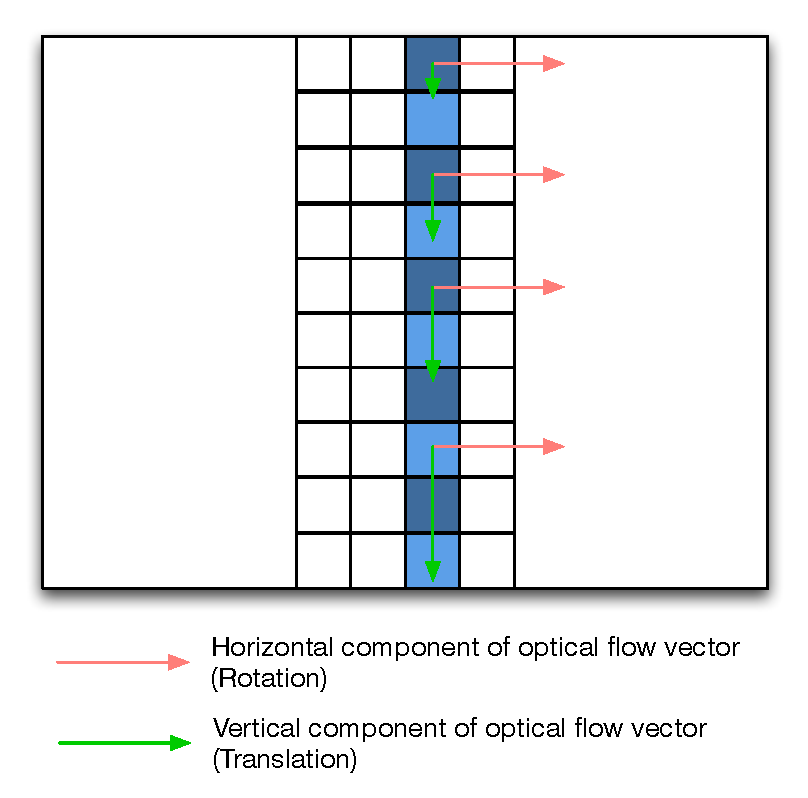
\includegraphics[scale=0.3]{rotation_diag}
\caption{Diagram demonstrating the expected difference in behaviour between the separated vertical and horizontal components of observed optical flow vectors calculated from \textbf{\textit{forward-turning motion}}.}
  \end{figure}
  
  
\end{frame}

\begin{frame}[fragile]
  \frametitle{Robot Speed}
  
\vspace{-10pt}

By recording multiple ``calibration" models at different speeds, it should be possible to later infer the current speed using the standard \textit{speed-distance-time} equation.

  \begin{figure}[ht!]
\centering
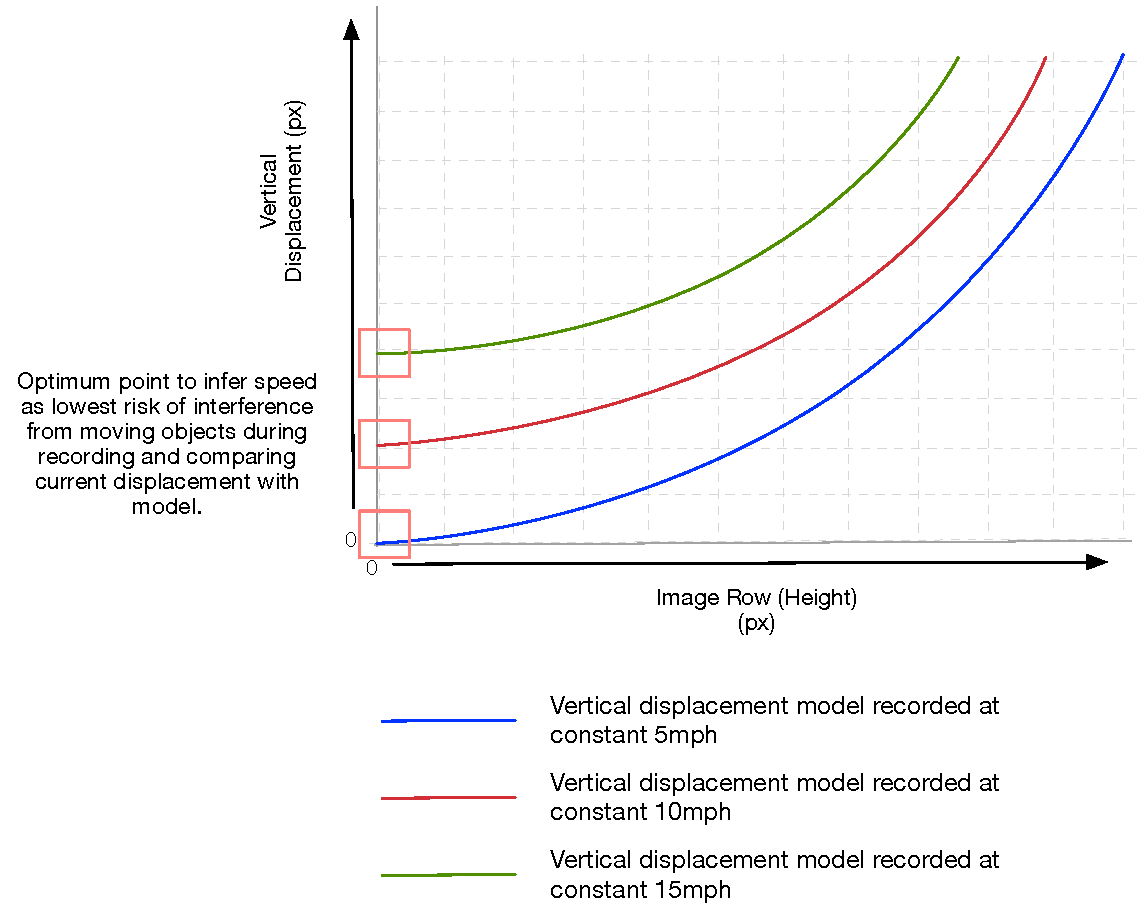
\includegraphics[scale=0.3]{speed_graph}
\caption{Diagram indicating examples of alternative vertical displacement models calculated while travelling at different constant speeds.}
  \end{figure}
  
  
\end{frame}

\begin{frame}[fragile]
  \frametitle{Investigation Aims}

  \begin{block}{Primary Aims}
  
  	  \begin{enumerate}[label={\arabic*.}]
  \item Establish which out the following appearance-based template matching similarity measures:
 {\small \begin{itemize}[label={\textbullet}]
  	\item Euclidean Distance
  	\item Correlation Coefficient
  	\item Histogram Correlation
  	\item Histogram Chi-Square
  \end{itemize} }
  
  best supports the predicted positive correlation between the vertical position of features within an image, and the level of vertical displacement demonstrated.
 
  \item Use the generated model of vertical displacement to identify potential obstacles and changes in terrain gradient based upon the predicted ‘comparative trend’ behaviour.
\end{enumerate}

  \end{block}

\end{frame}

\begin{frame}[fragile]
  \frametitle{Investigation Aims}

  \begin{block}{Secondary Aims}
  
  	  \begin{enumerate}[label={\arabic*.}]
  	  
  \item Further extend the capabilities of the vertical displacement model to provide estimates into the current speed of travel demonstrated by the robot.

  \item Add support for providing an estimation into the change in orientation.
 
\end{enumerate}

  \end{block}

\end{frame}

\plain{Experiment Methods}

\begin{frame}[fragile]
  \frametitle{Gathering Datasets}
  
  No existing imagery datasets were found to be suitable, therefore new sets had to be collected.
  
  \vspace{5pt}
  
    \begin{figure}[ht!]
\centering
\includegraphics[scale=0.05]{rig_setup}
\caption{Camera-rig setup used to capture the experiment datasets from front and back profiles.}
  \end{figure}
  
\end{frame}

\begin{frame}[fragile]
  \frametitle{Gathering Datasets}
  
  Images taken at a number of locations, but \textbf{four} were eventually selected based upon their variety in terms of \textbf{terrain texture} and \textbf{lighting conditions}.
  
  \vspace{15pt}
  
    \begin{figure}[ht!]
\centering
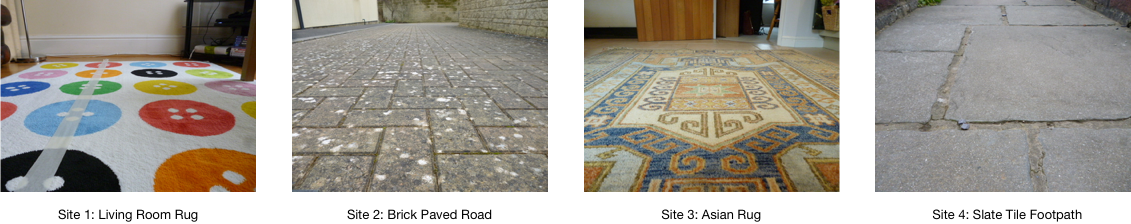
\includegraphics[scale=0.27]{locations}
\caption{Examples of the first frame captured from each of the four location datasets.}
  \end{figure}
  
\end{frame}

\begin{frame}[fragile]
  \frametitle{Experiment Methods}
  
  {\normalsize Over time, \textbf{investigation focus changed} from exploring a series of reasonably ``generalised" research aims, to instead concentrating almost exclusively on one small, but very important aspect; 
  \vspace{-10pt}
  
  \begin{block}{}
  \textit{Ensuring that accurate results for appearance-based motion displacement could continue to be achieved, across terrain lacking any significant features and/or demonstrating highly repetitive patterns}.
  \end{block}}
		
  \begin{block}{Three Experiments}
  \begin{enumerate}[label={\arabic*.}]
  	  
  \item Template Matching - \textbf{Multiple Small Patches}

  \item Template Matching - \textbf{Full-width Patches (Non-Scaled)}
  
  \item Template Matching - \textbf{Full-width Patches (Geometrically Scaled)}
 
\end{enumerate}
\end{block}

\end{frame}

\begin{frame}{Experiment One - Multiple Small Patches}

%Input: Two images with a set displacement between them (e.g. 10cm). \\

\textbf{Stage One} \\ \vspace{0.2cm}

Import two consecutive images, and convert from RGB (BGR in OpenCV) colour space to HSV.

\begin{figure}[ht!]
\centering
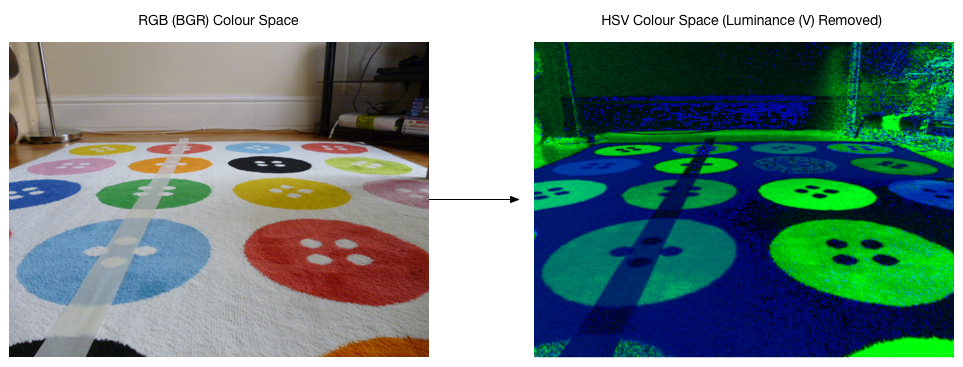
\includegraphics[scale=0.26]{rgb2hsv.png}
  \end{figure}
  
The 'V' channel is then removed in order to improve robustness to lighting changes between frames. 
\end{frame}

\begin{frame}{Experiment One - Multiple Small Patches}

\textbf{Stage Two} \\ \vspace{0.2cm}

Extract a percentage-width region of interest (ROI) from centre of first image.

\begin{figure}[ht!]
\centering
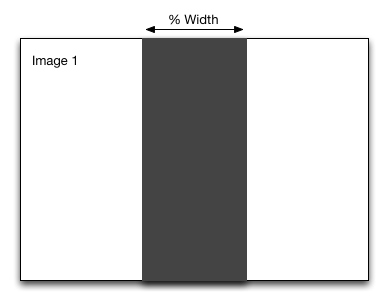
\includegraphics[scale=0.5]{stage1.png}
  \end{figure}
  
\end{frame}

\begin{frame}{Region-of-Interest}

\textbf{Why do we need to extract a ROI?} \\ \vspace{0.5cm}

\textbf{Focus-of-expansion}: Objects in images do not actually move in 1-dimension (i.e. straight down the image). \\ \vspace{0.2cm}

This effect is minimised towards the centre of the image.

\begin{figure}[ht!]
\centering
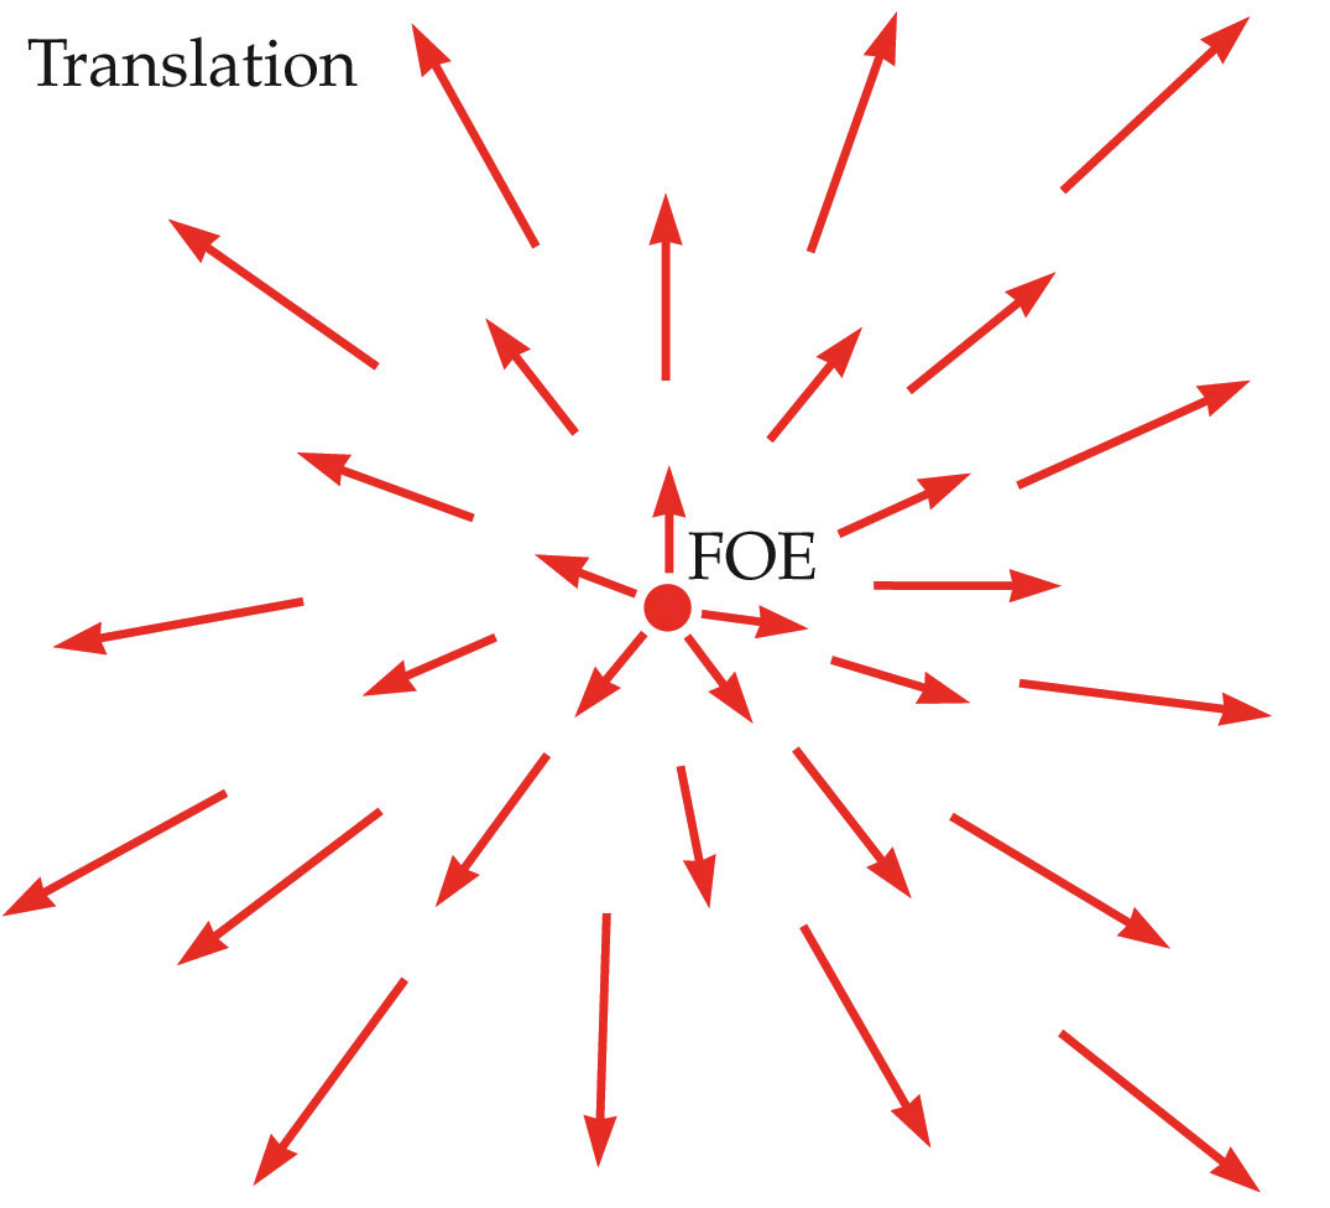
\includegraphics[scale=0.15]{foe.png}
\caption{Diagram indicating the perceived effects caused by Focus of Expansion. Courtesy: [5]}
  \end{figure}
  
\end{frame}

\begin{frame}{Experiment One - Multiple Small Patches}

\textbf{Stage Three} \\ \vspace{0.2cm}

Extract patches of a fixed size around each pixel within the extracted ROI.

\begin{figure}[ht!]
\centering
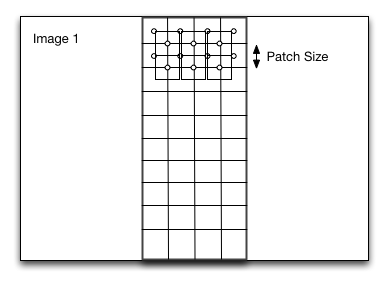
\includegraphics[scale=0.4]{stage2.png}
\caption{\textbf{Simplified} example of patch extraction within ROI.}
  \end{figure}
  
\end{frame}

\begin{frame}{Experiment One - Multiple Small Patches}

\textbf{Stage Four} \\ \vspace{0.2cm}

For each patch extracted from \emph{image one}, move down through a localised search window (column) in \emph{image two} searching for the best match against the template patch. 

\begin{figure}[ht!]
\centering
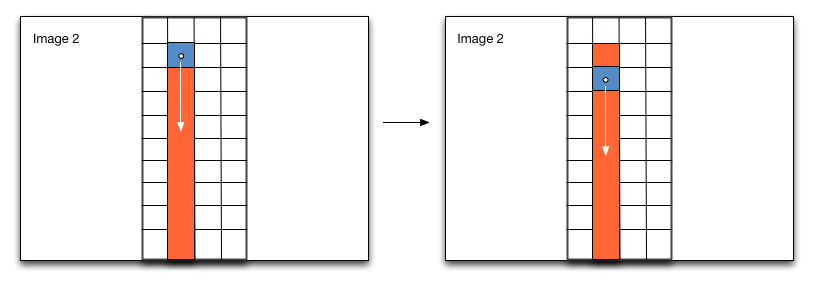
\includegraphics[scale=0.35]{stage3.png}
\caption{Example of ``best match" search within local column.}
\end{figure}
  
\end{frame}

\begin{frame}{Experiment One - Multiple Small Patches}

\textbf{Stage Five} \\ \vspace{0.2cm}

Identify the patch within the localised search window that provides the ``best match" via correlation-based matching (e.g. Euclidean Distance, SSD or Correlation coefficient). 

\begin{figure}[ht!]
\centering
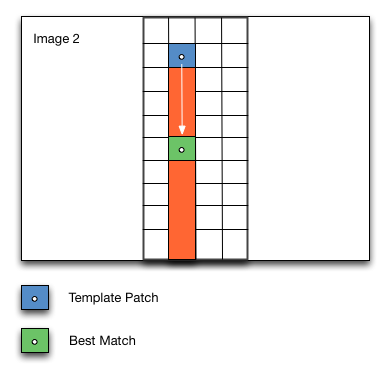
\includegraphics[scale=0.35]{stage4.png}
\end{figure}

\end{frame}

\begin{frame}{Experiment One - Multiple Small Patches}

\textbf{Stage Six} \\ \vspace{0.2cm}

Average all measured displacements for each pixel along a given row.

\begin{figure}[ht!]
\centering
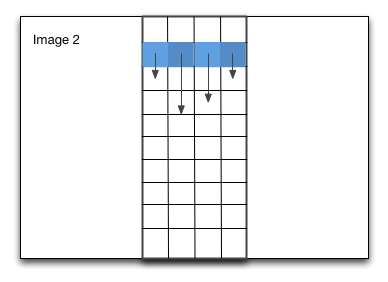
\includegraphics[scale=0.4]{stage5.png}
\end{figure}

Outliers are removed by ignoring any displacements that lie outside of (2 x Standard Deviation) of the mean.

\end{frame}

\begin{frame}{Experiment One - Multiple Small Patches}

\textbf{Repeat Stages 1-6} \\ \vspace{0.2cm}

Repeat stages 1-6 for an entire collection of ``calibration" images taken of \emph{flat, unobstructed} terrain.

\begin{figure}[ht!]
\centering
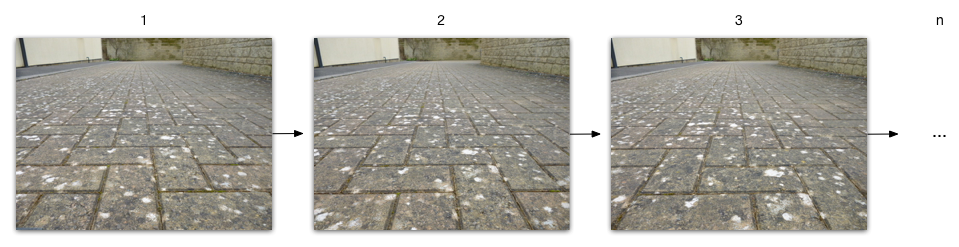
\includegraphics[scale=0.3]{calibimages.png}
\end{figure}

\end{frame}

\begin{frame}{Experiment One - Multiple Small Patches}

\textbf{Stage Seven} \\ \vspace{0.2cm}

Plot the \emph{average displacement} for each ROI row, calculated from the displacements recorded over all calibration images.

\begin{figure}[ht!]
\centering
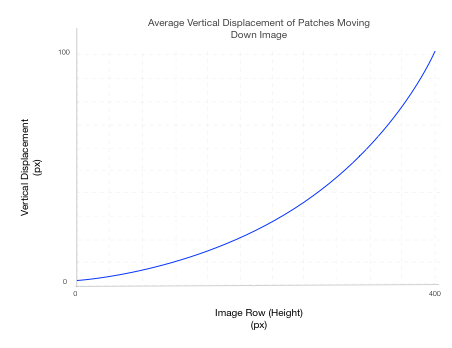
\includegraphics[scale=0.45]{graph.png}
\end{figure}

\end{frame}

\begin{frame}{Experiment Two - Full-width Patches (Non-Scaled)}

\begin{block}{Focus}

Establishing if adopting \textbf{\textit{larger}} patches in fewer numbers provided better appearance-based matching accuracy than using many more, but critically much \textbf{\textit{smaller}} overlapping patches.
	
\end{block}

While the underlying method remained the same as in the first experiment, some key changes were made:

 \begin{itemize}[label={\textbullet}]
  	\item Extracting a central region of interest relative to the \textbf{ground plane}, as opposed to extracting a fixed-width column from the image plane.
  	\item Moving away from multiple overlapping small patches, in favour of adopting a single, \textbf{full-width} patch to represent a single row in the image.
  \end{itemize}

\end{frame}

\begin{frame}[fragile]
  \frametitle{Exhaustive vs. Non-Exhaustive Search}
  
  \vspace{-10pt}
  
  Issue discovered regarding the use of \textbf{non-exhaustive} searching causing erroneous results. All tests in experiments two and three were conducted using both exhaustive and non-exhaustive approaches.
  
  \vspace{-10pt}

  \begin{figure}[ht!]
\centering
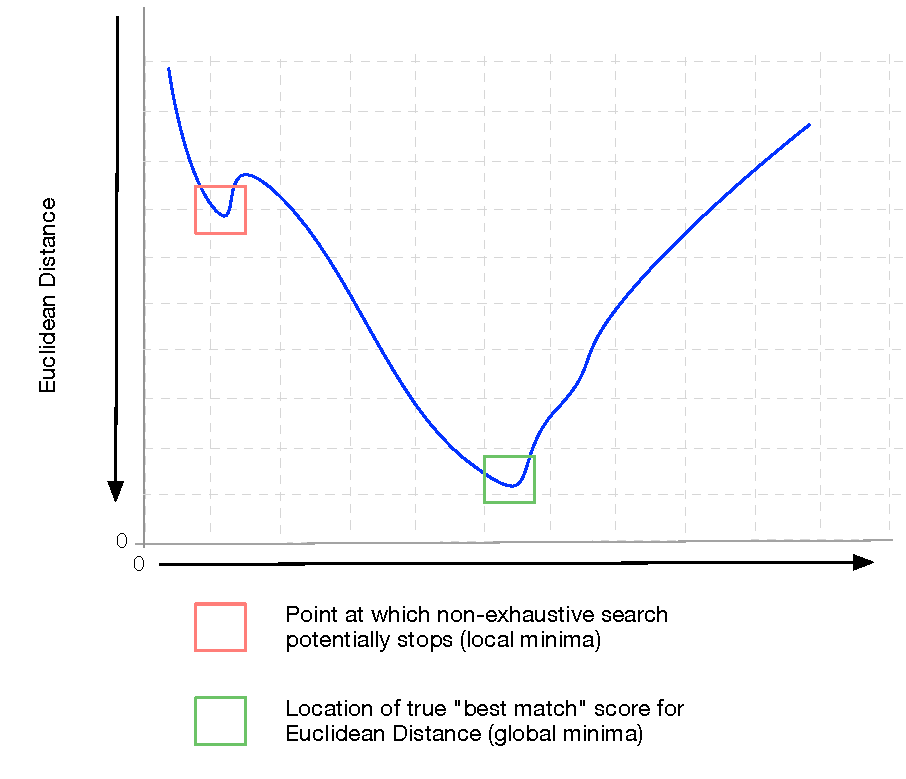
\includegraphics[scale=0.32]{ed}
 \vspace{-5pt}
\caption{Example of potential early termination of non-exhaustive search due to entering local minima caused by noise, rather than global minima which represents to true best match.}
\end{figure}

\end{frame}

\begin{frame}{Perspective Distortion Calibration Tool}

\vspace{-5pt}

To extract a region-of-interest along the \textit{ground plane}, the system would need to take account of \textbf{perspective distortion}. Therefore, a simple \textbf{calibration tool} was implemented, enabling users to define the required region of interest within an image.

 \begin{figure}[ht!]
\centering
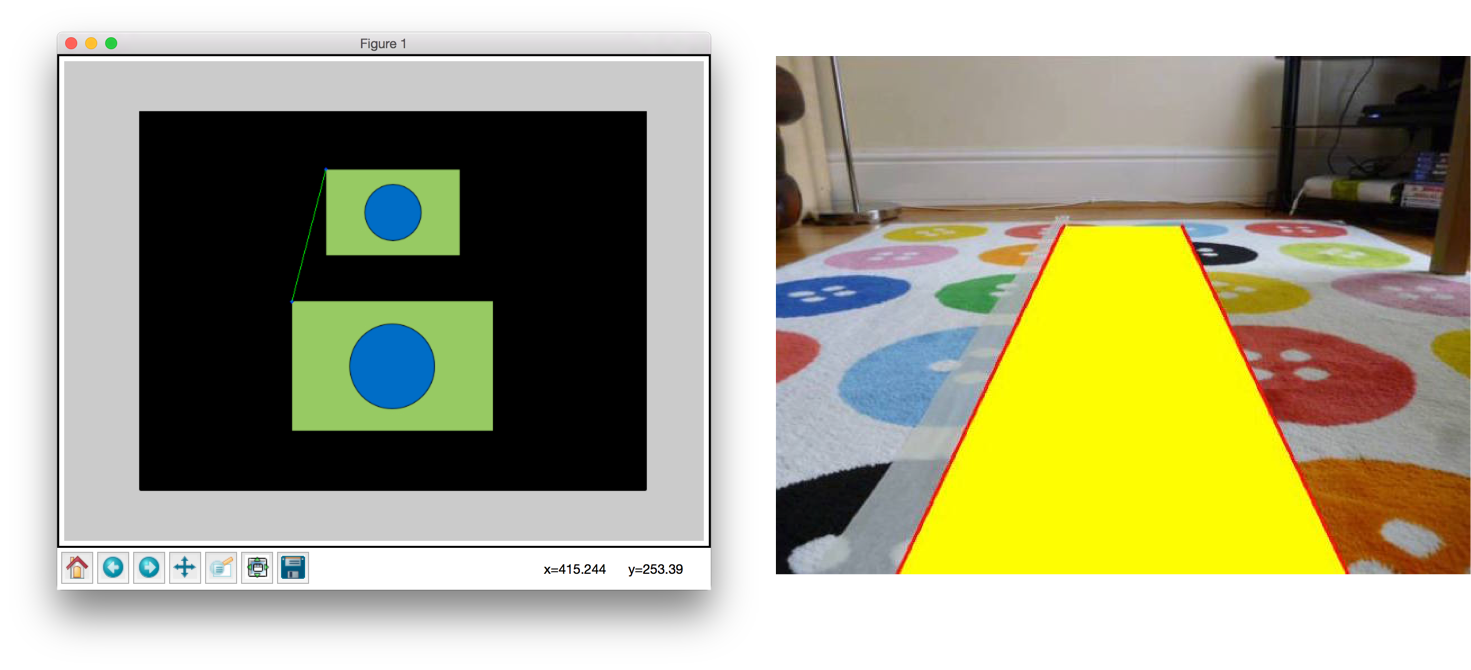
\includegraphics[scale=0.16]{calib_tool}
\vspace{-10pt}
 \caption{Results of the verification test for the approach towards geometric scaling of template patch pixel coordinates.}
\end{figure}

\end{frame}


\begin{frame}{Experiment Three - Full-width Patches (Scaled)}

\begin{block}{Focus}

Add \textbf{geometric scaling} of template patch in order to account for objects appearing larger as they approach the camera. 
	
\end{block}
 \vspace{15pt}
  \begin{figure}[ht!]
\centering
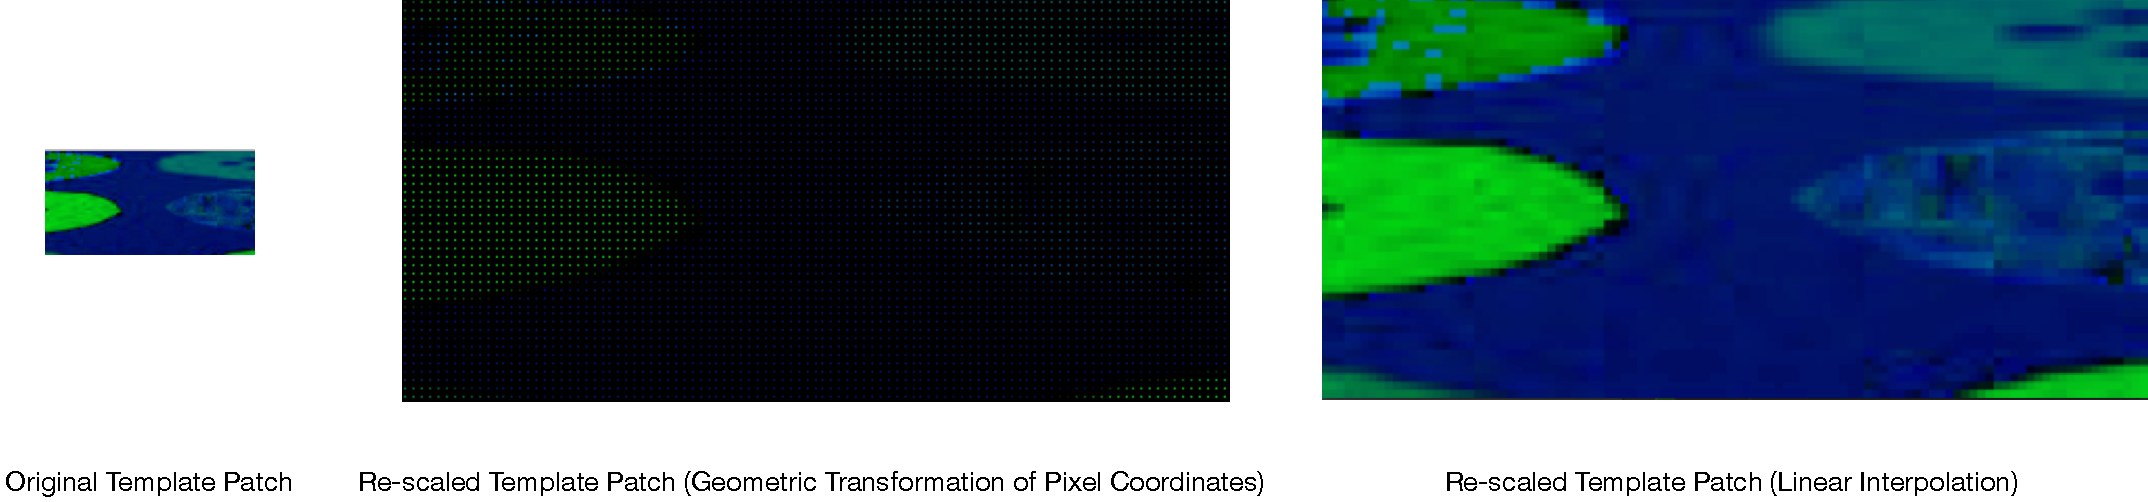
\includegraphics[scale=0.28]{scaling_types}
 \caption{Comparison between various approaches of performing scaling of the original template patch image. In the case of linear interpolation, additional information has been added to image as a result of “estimating” the colour that lies between two original pixels.}
\end{figure}

\end{frame}


\begin{frame}{Experiment Three - Full-width Patches (Scaled)}

\vspace{-5pt}
\begin{block}{6 Stage Process}
  \vspace{-5pt}
{\small \begin{enumerate}[label={\arabic*.}]
  \item Obtain the width and height of the current template patch.
  \item Obtain the calibrated width of the search window with respect to the current image row.
  \item Calculate the independent scale factor for the width and height between the template patch and the search window.
  \item Treating each pixel as a 2D coordinate in geometric space, scale the position of each pixel coordinate within the template patch relative to the position of centre coordinate.
  \item For each scaled pixel coordinate, extract the value of the pixel at the corresponding position with the search window and add to a temporary “image” data structure.
  \item Perform template matching between the original template patch, and the new ``extracted" temporary image.
 
\end{enumerate}}
	
\end{block}

\end{frame}


\begin{frame}{Experiment Three - Full-width Patches (Scaled)}
	
	\vspace{-5pt}
  \begin{block}{Testing of Scaling Approach} A simple test was devised to confirm geometric scaling worked as expected under ``perfect" conditions.
 \vspace{-15pt}
  		  \begin{figure}[ht!]
\centering
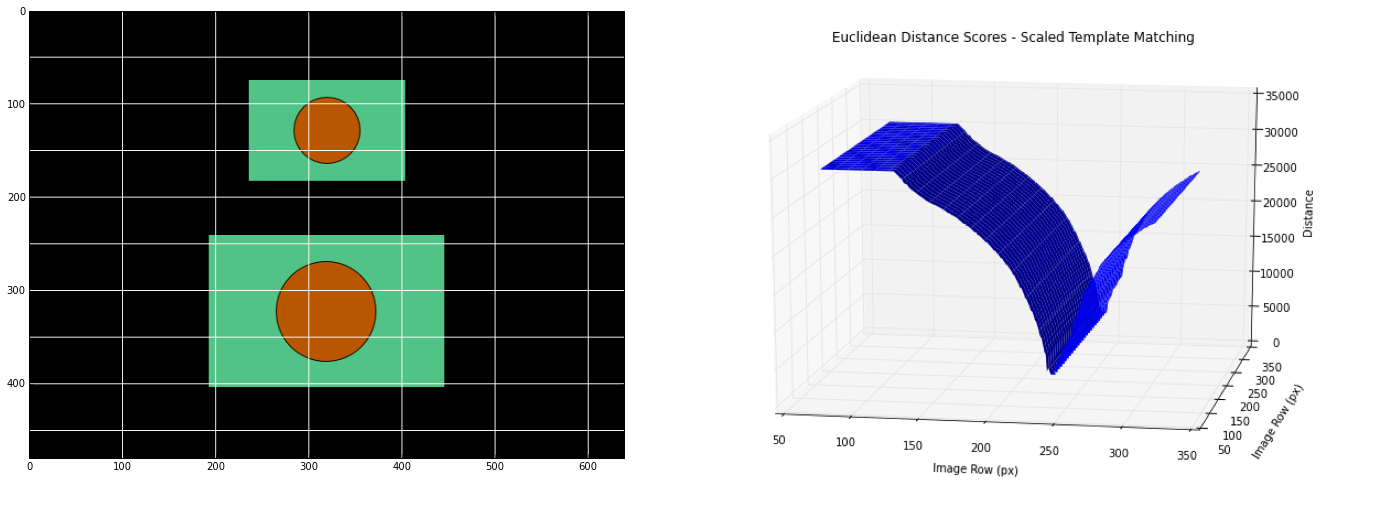
\includegraphics[scale=0.23]{scaling_verif}
 \caption{Results of the verification test for the approach towards geometric scaling of template patch pixel coordinates.}
\end{figure}
  		
  \end{block}


\end{frame}

\begin{frame}{Additional Experimental Work}

\vspace{-10pt}

{\small Some additional experimental work was conducted as part of the larger project investigation, but these did not actively contribute to the final investigation results.

\begin{itemize}[label={\textbullet}]
  	\item Investigation of Campbell \textit{et al.} [1] approach to feature tracking to provide optical flow field (based heavily upon C\# implementation provided by Dr. Rainer Hessmer (\href{http://www.hessmer.org/blog/2010/08/17/monocular-visual-odometry}{Source}))
  	\item Investigation of edge-based template matching discussed by Perveen \textit{et al.} [3]
  \end{itemize} }
  
  \vspace{-10pt}
  
    		  \begin{figure}[ht!]
\centering
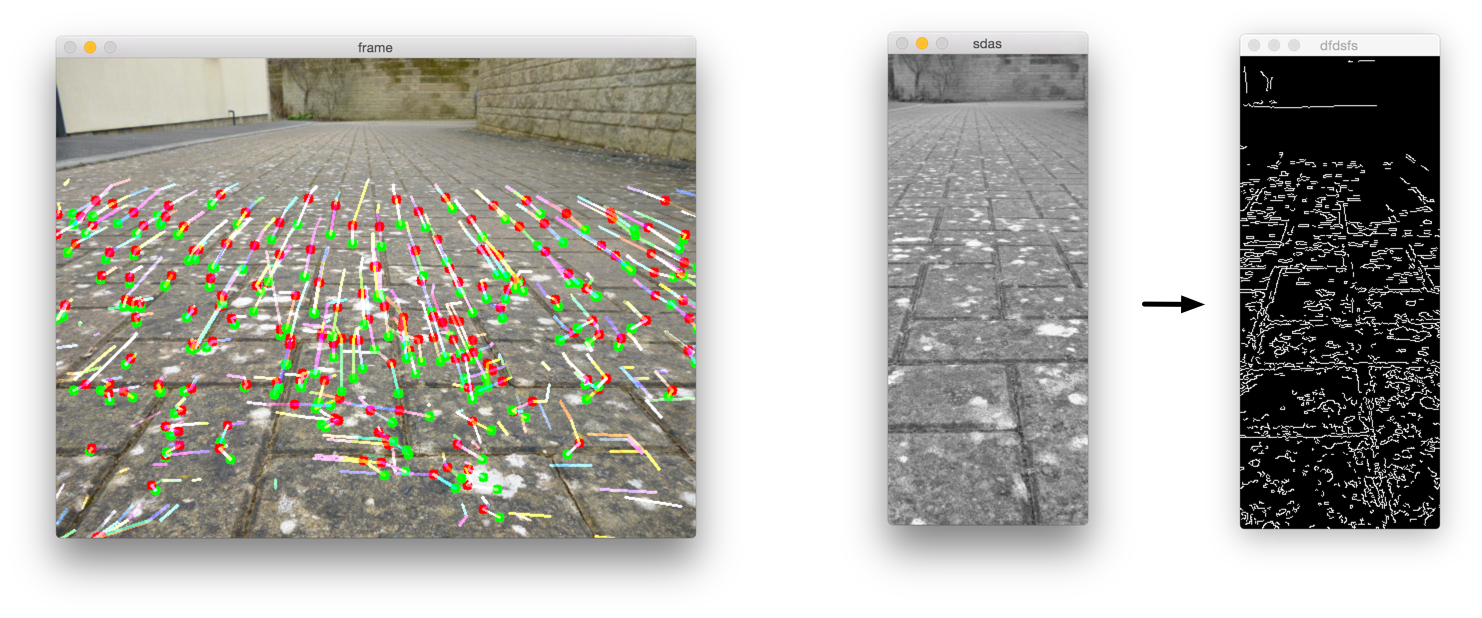
\includegraphics[scale=0.13]{additional_work}
 \caption{\textbf{Left:} Example of feature tracking to establish optical flow field. \textbf{Right:} Edge-based template matching using Canny edge detector.}
\end{figure}
  		

\end{frame}

\plain{Investigation Results\\ \vspace{0.2cm} \footnotesize{\href{http://nbviewer.ipython.org/github/cgddrd/CS39440-major-project/tree/develop/src/template_matching_scaling/notebooks}{View Results (Courtesy: nbviewer)}}}

\begin{frame}{Results}

Results can be described as generally \textbf{inconclusive}. \\ \vspace{0.5cm}

However from the results obtained, we have learned:

\begin{enumerate}[label={\arabic*.}]
  \item Under certain terrain conditions, it is possible to potentially establish a relationship between row height in an image, and average downwards pixel displacement. \vspace{0.5cm} 
  \item The performance of each appearance-based similarity measure can vary widely, based upon factors including:
 \vspace{0.2cm} 
  \begin{itemize}[label={\textbullet}]
  	\item \textbf{Terrain texture} (e.g. highly patterned, isotropic or homogenous)
  	\item \textbf{Patch size} (Balance between reducing ``noise" and representing true displacement behaviour)
  	\item \textbf{Exhaustive vs. Non-exhaustive search}
  	\item \textbf{Scaling vs. Non-scaling}
  \end{itemize}
\end{enumerate}

\end{frame}

\begin{frame}{Results: Approach Comparison - `Living Room Rug' Dataset}

\begin{figure}[ht!]
\centering
\vspace{-0.5cm}
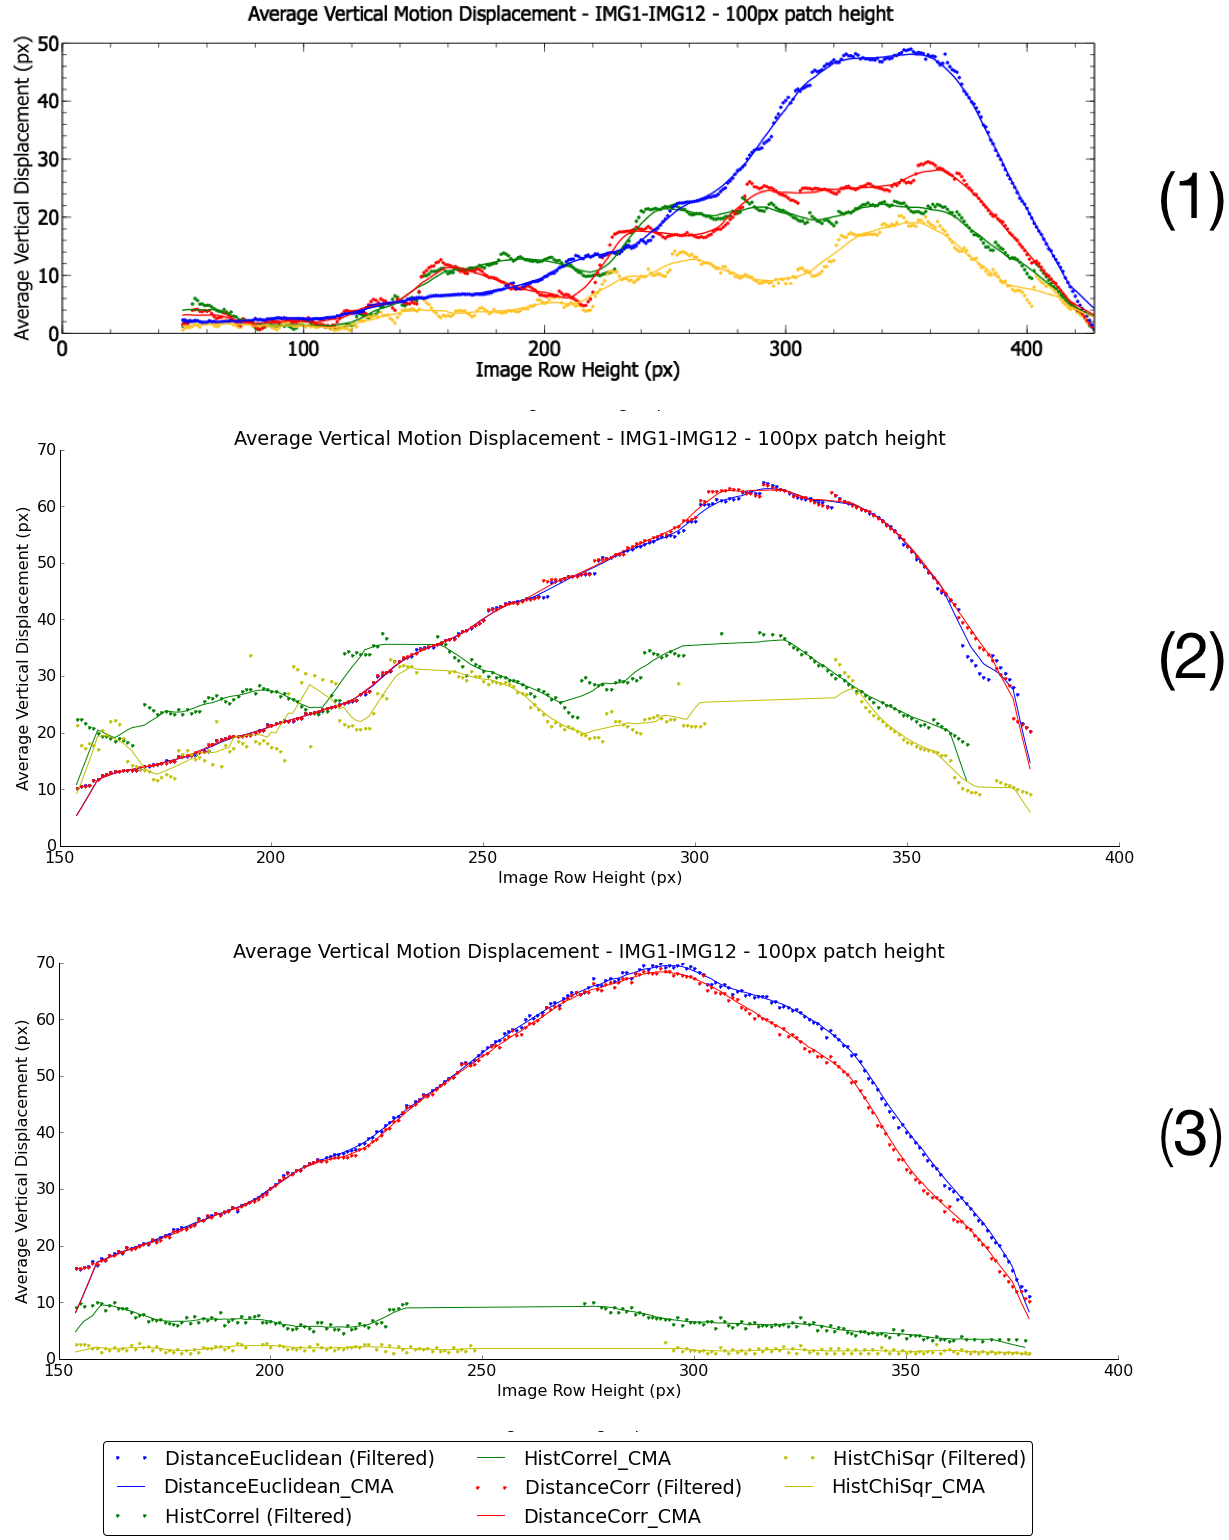
\includegraphics[scale=0.12]{flat_pres_results.png}
\caption{Comparison of results for the `Living room rug' dataset using an exhaustive search and 100px patch size. Small patches (Graph 1), full-width patches (Graph 2) and geometrically scaled full-width patches (Graph 3).}
\end{figure}

\end{frame}

\begin{frame}{Results: Approach Comparison - `Brick-paved Road' Dataset}

\begin{figure}[ht!]
\centering
\vspace{-0.5cm}
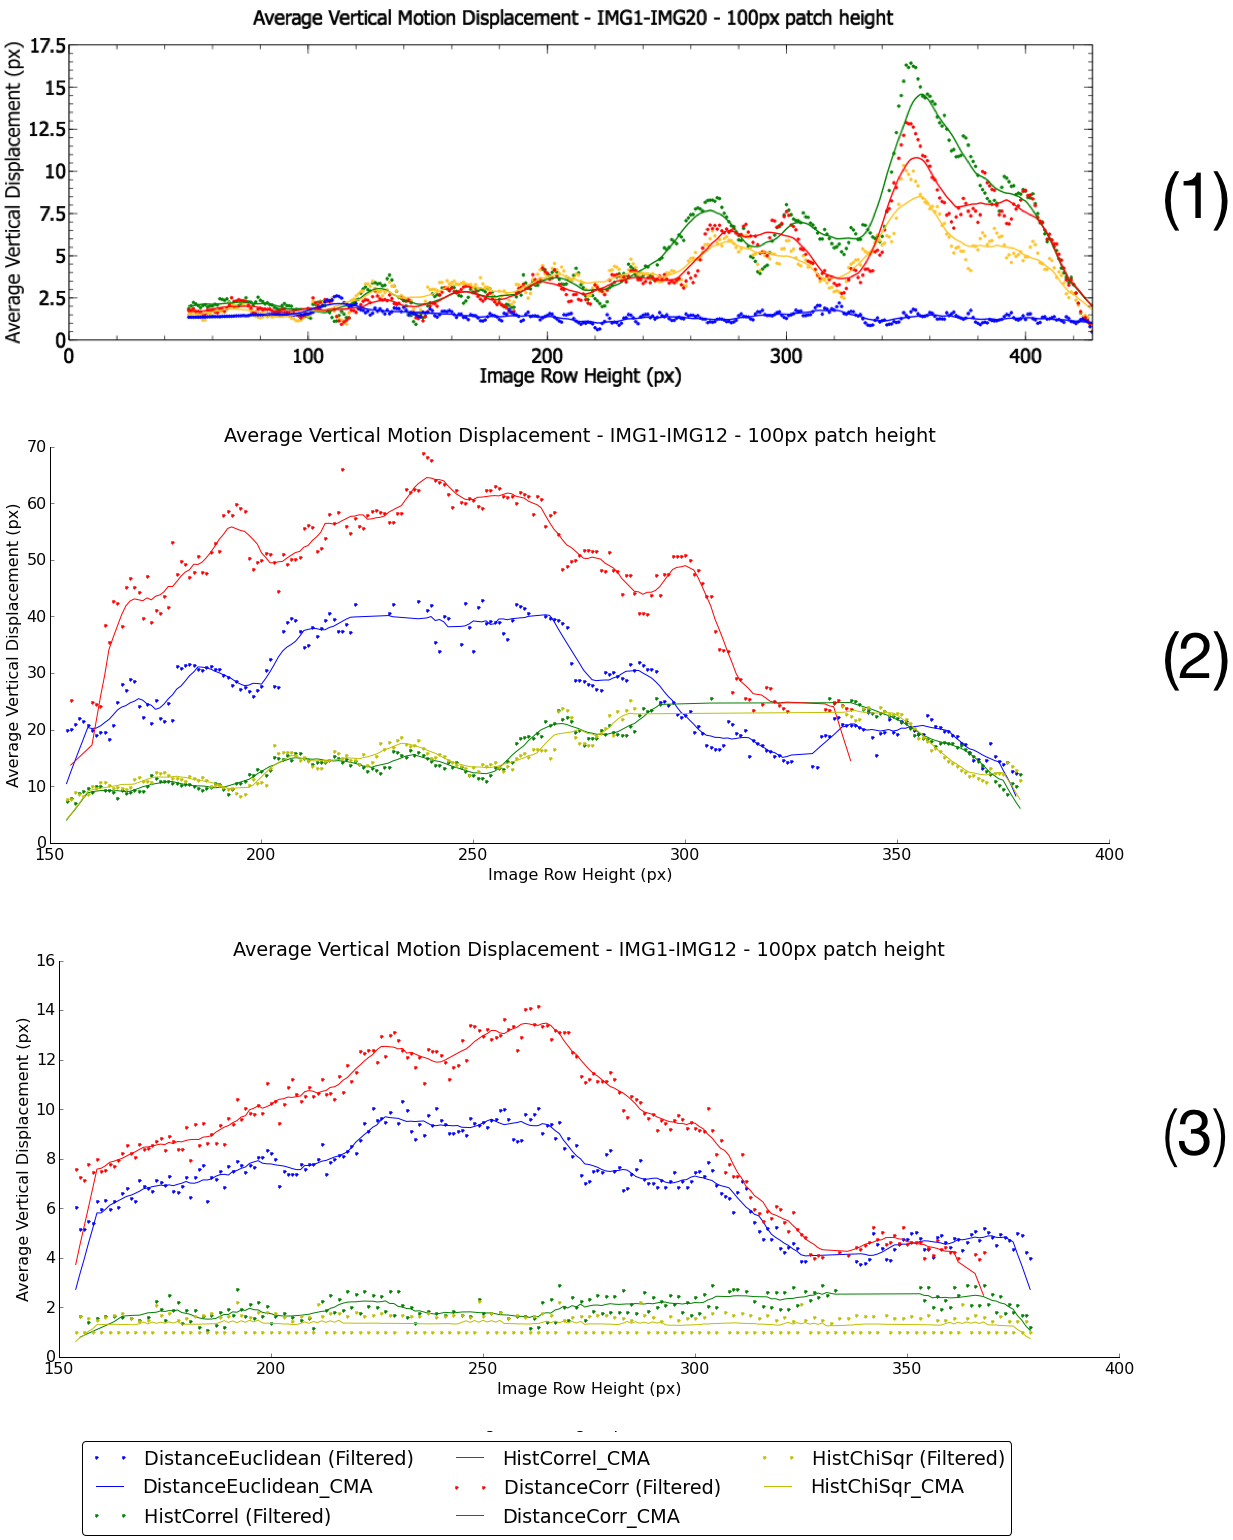
\includegraphics[scale=0.12]{outside_pres_results.png}
\caption{Comparison of results for the `Brick-paved road' dataset using an exhaustive search and 100px patch size. Small patches (Graph 1), full-width patches (Graph 2) and geometrically scaled full-width patches (Graph 3).}
\end{figure}


%\begin{columns}[T] % align columns
%\begin{column}{.48\textwidth}
%
%\textbf{Input Collection:}
%
%\begin{figure}[ht!]
%\centering
%\vspace{0.3cm}
%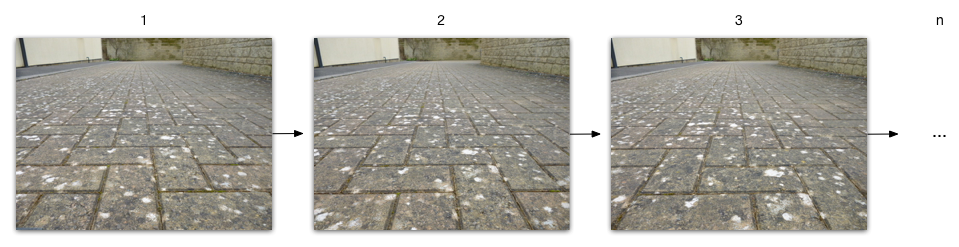
\includegraphics[scale=0.18]{calibimages.png}
%\end{figure}
%
%\end{column}%
%\hfill%
%\begin{column}{.48\textwidth}
%
%\textbf{Result:}
%\begin{figure}[ht!]
%\centering
%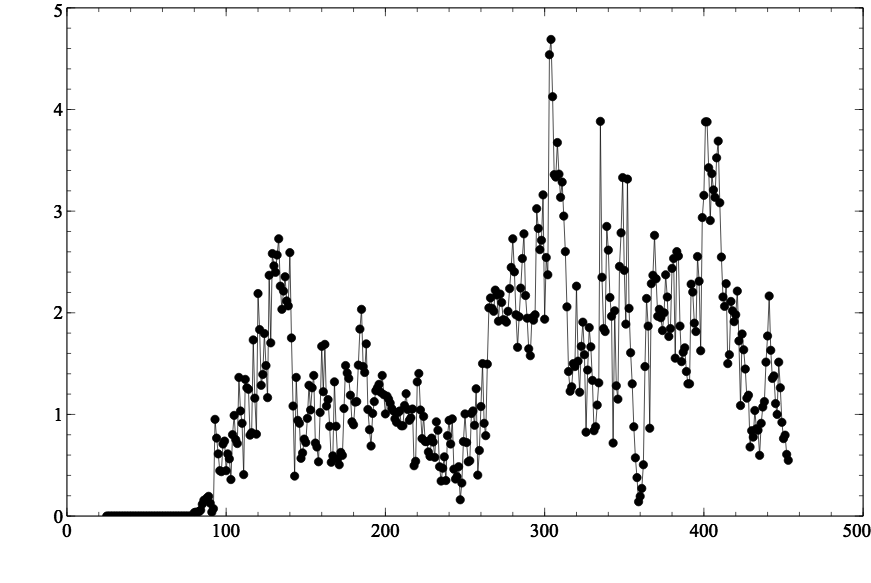
\includegraphics[scale=0.22]{wiltshire_outside_10cm.png}
%\end{figure}
%
%\end{column}%
%\end{columns}

\end{frame}

\begin{frame}{Results: Exhaustive vs. Non-Exhaustive Search}

%\begin{figure}[ht!]
%\centering
%\vspace{-0.5cm}
%\includegraphics[scale=0.12]{ }
%\caption{Comparison of results for the `Brick-paved road' dataset using an exhaustive search and 100px patch size. Small patches (Graph 1), full-width patches (Graph 2) and geometrically scaled full-width patches (Graph 3).}
%\end{figure}

\vspace{-0.4cm}

\begin{columns}[T] % align columns
\begin{column}{.48\textwidth}

\textbf{Non-Exhaustive}

\begin{figure}[ht!]
\centering
\vspace{0.1cm}
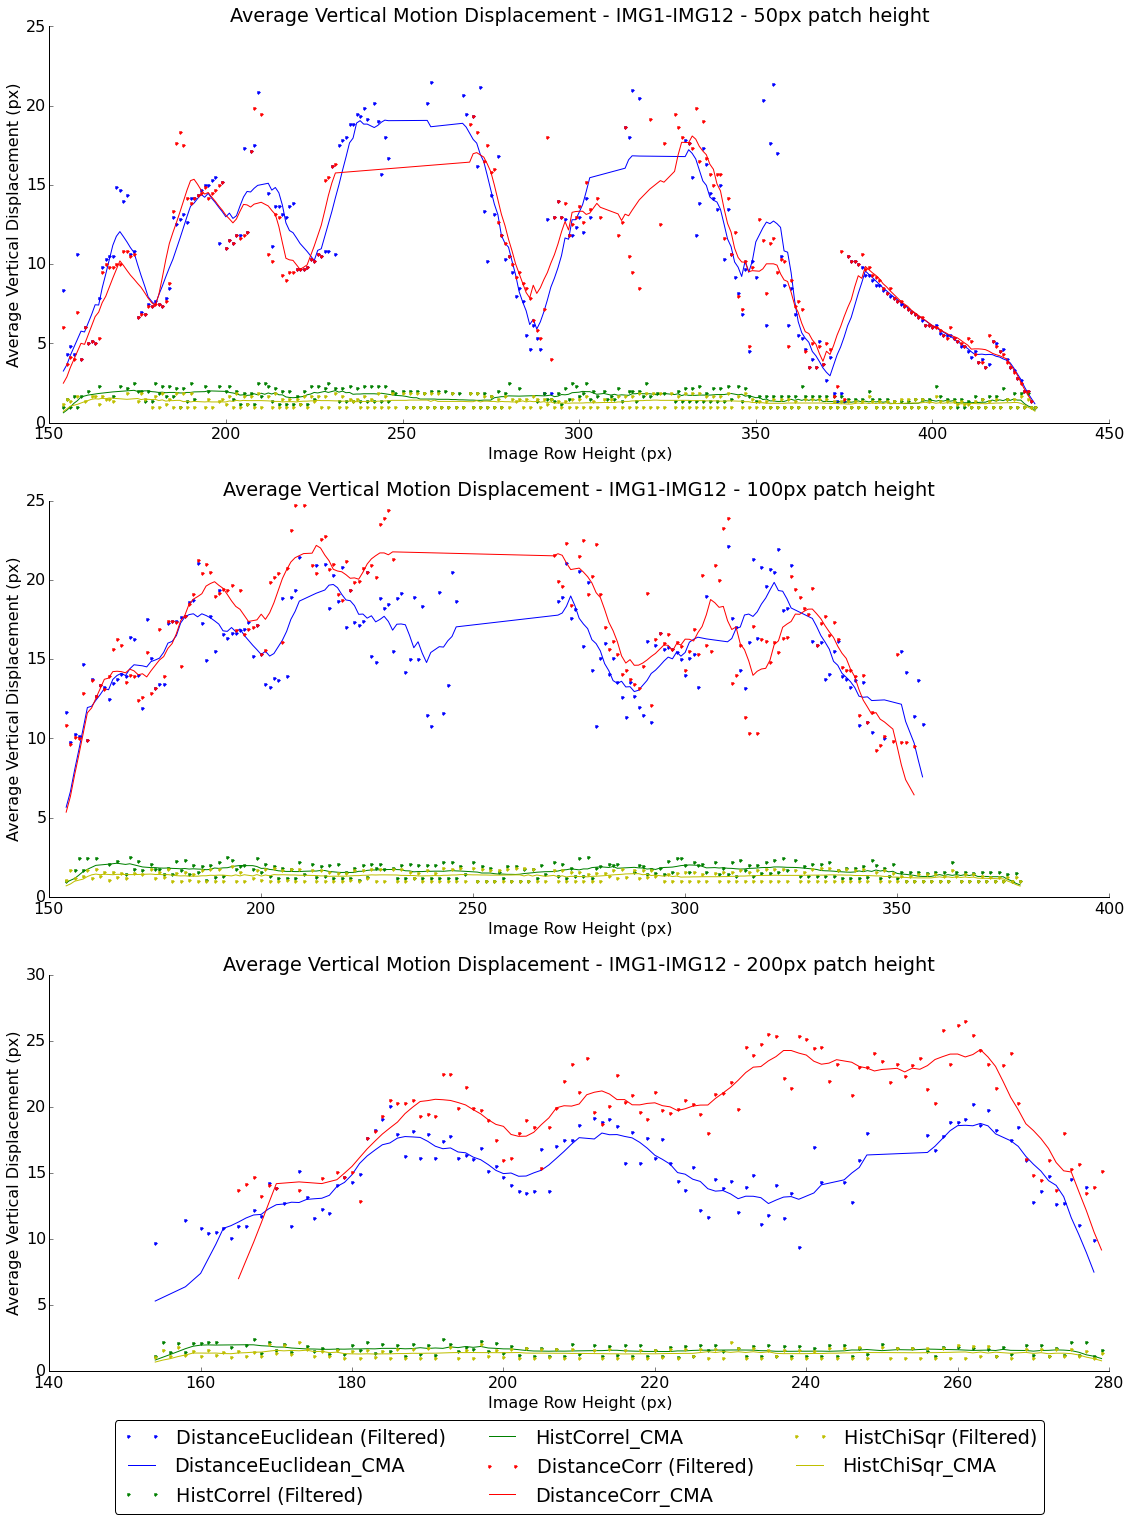
\includegraphics[scale=0.11]{flat_10cm_scaled}
\end{figure}

\end{column}%
\hfill%
\begin{column}{.48\textwidth}

\textbf{Exhaustive}
\begin{figure}[ht!]
\centering
\vspace{0.1cm}
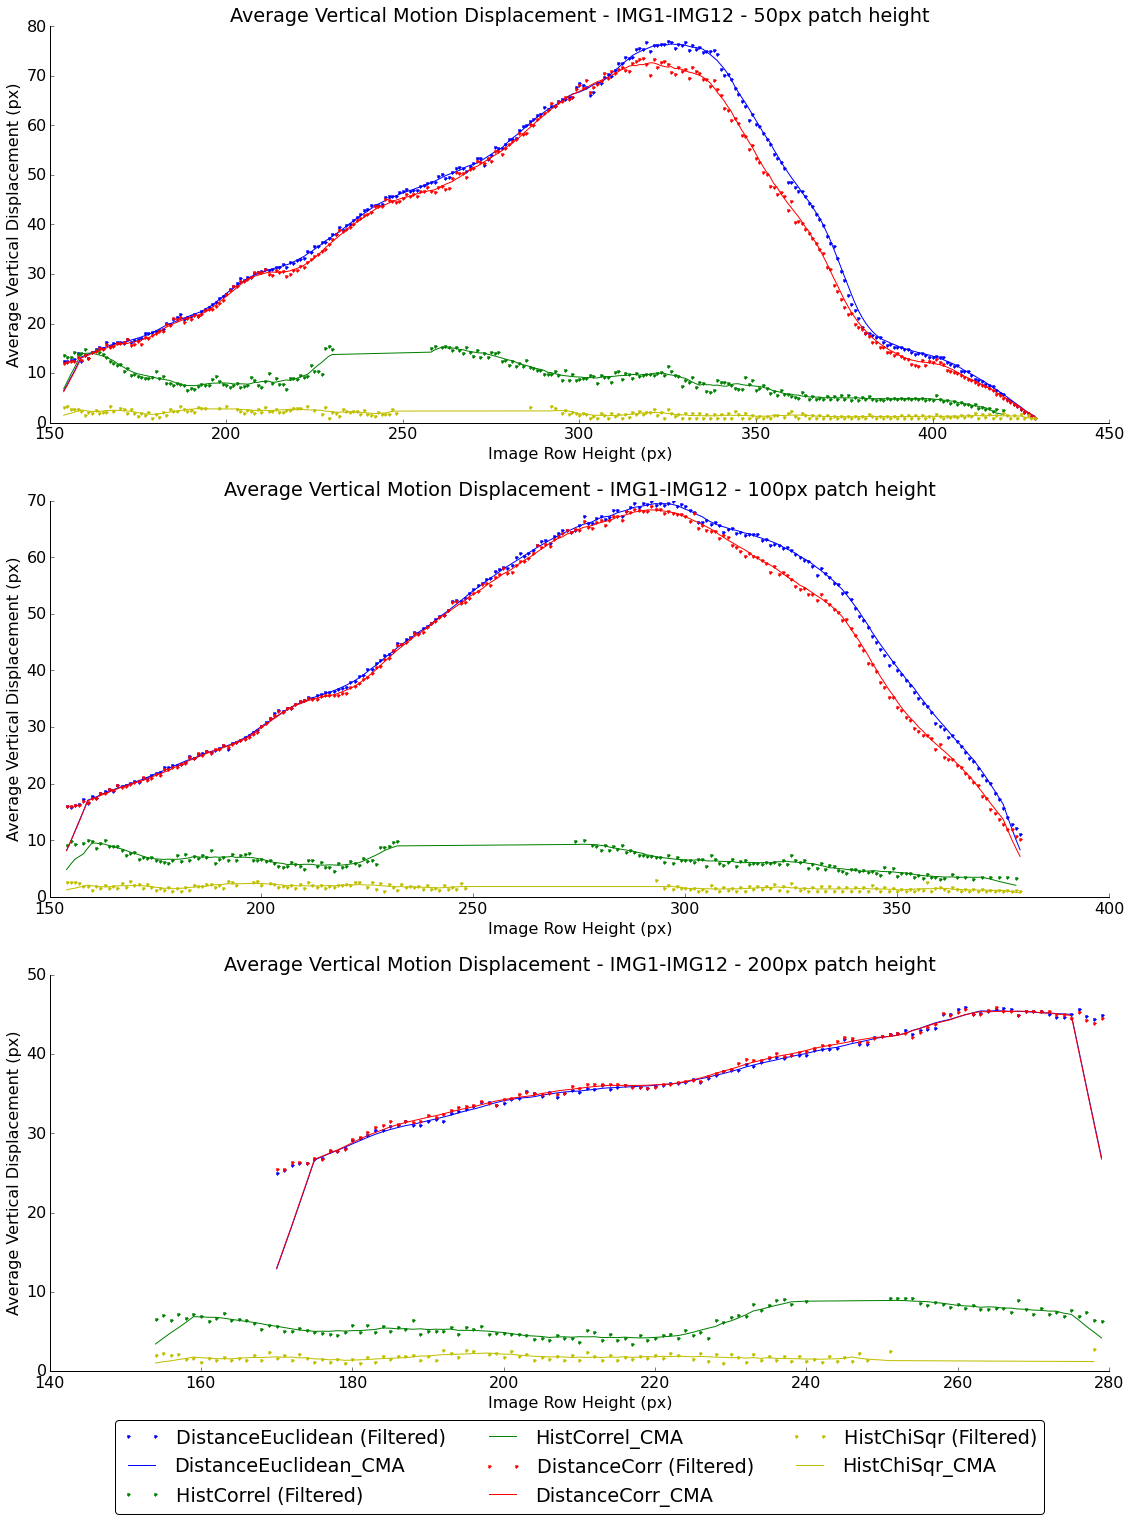
\includegraphics[scale=0.11]{flat_10cm_scaled_exhaustive}
\end{figure}

\end{column}%
\end{columns}

\begin{figure}[ht!]
\caption{Comparison between non-exhaustive and exhaustive search performance using geometrically scaled template patches and the `Living room rug' dataset.}
\end{figure}

\end{frame}

\begin{frame}{Results: Patch Size Comparison - `Slate Footpath' Dataset}

\begin{figure}[ht!]
\centering
\vspace{-0.5cm}
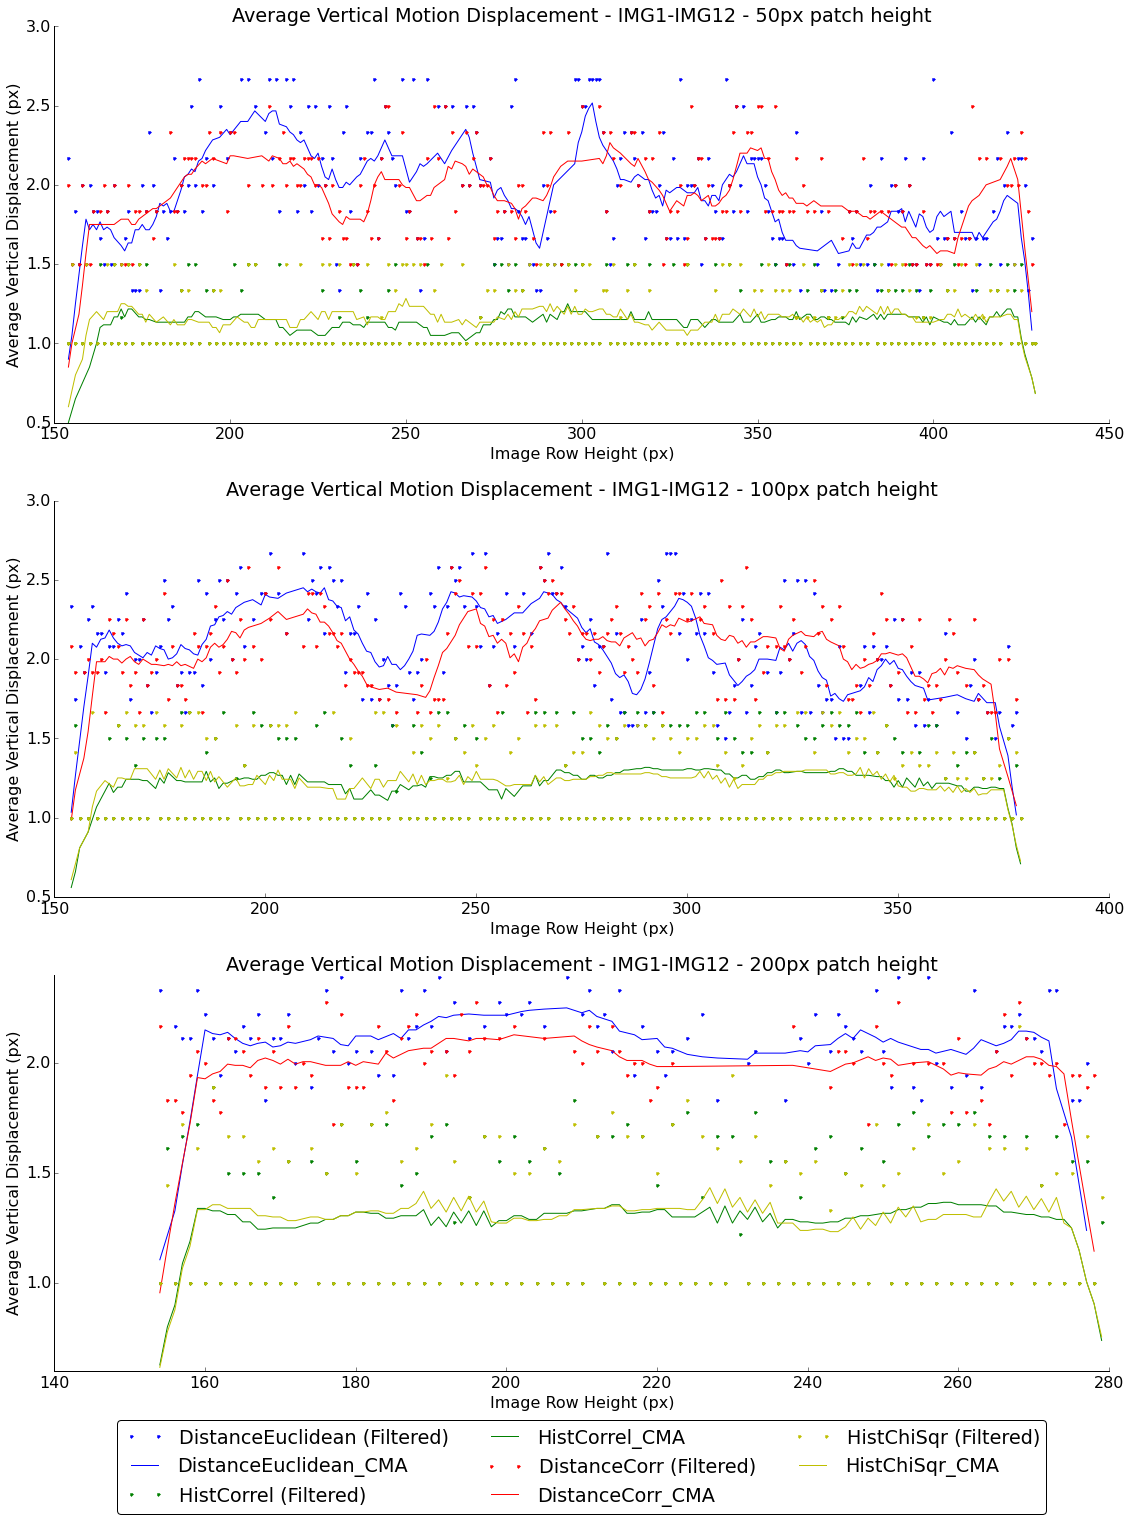
\includegraphics[scale=0.13]{path_outside_10cm_scaled.png}
\caption{Comparison of results for the `Living room rug' dataset using geometrically-scaled patches of 50px, 100px and 200px heights under an exhaustive search approach.}
\end{figure}

\end{frame}

\plain{Conclusion}

\begin{frame}[fragile]
  \frametitle{Future Work}

	Great potential for future work, most likely focussing on areas including:
	
	\begin{itemize}[label={\textbullet}]
  	\item Further experimentation to establish most appropriate combination of similarity-measure, search approach and patch size for a \textbf{given terrain type}. 
  	\item Development of a system to identify ``significant" changes in vertical displacement model that are potentially indicative of a potential obstacle or change in terrain gradient.
  	\item Development of system to estimate change in robot heading.
  	\item Development of system to estimate current robot speed.
  \end{itemize}
	
\end{frame}

\begin{frame}[fragile]
  \frametitle{Conclusion Summary}
  
	Project has laid the groundwork upon which further development can subsequently be conducted. \\ \vspace{0.2cm}
	
	While not all of the original aims were accomplished, research efforts had to be focussed on confirming the underlying hypothesis, which as a general concept, has been proven. \\ \vspace{0.2cm}
	
	\textbf{Not one single approach or solution will suffice for all terrain conditions.}

\end{frame}


%\begin{frame}{Project Management}
%
%Project is adopting a SCRUM-based approach to project management. \\ \vspace{0.2cm}
%
%\begin{itemize}
%	\item \textbf{Releases} - Major feature sets (e.g. work up to mid-project demo)
%	\item \textbf{Sprints} - Weekly time-boxed portion of work effort.
%	\item \textbf{Sprint Review \& Retrospectives} - Conducted as part of weekly project meeting with tutor. 
%\end{itemize}
%
%
%\textbf{Tools:} \textit{Github Issues} with \textit{\href{http://waffle.io}{Waffle.io}} (KANBAN), \textit{\href{http://burndown.io/}{Burndown.io}} (Burndown charts).
%	
%\end{frame}
%
%\begin{frame}{Project Management}
%
%\begin{figure}[ht!]
%\centering
%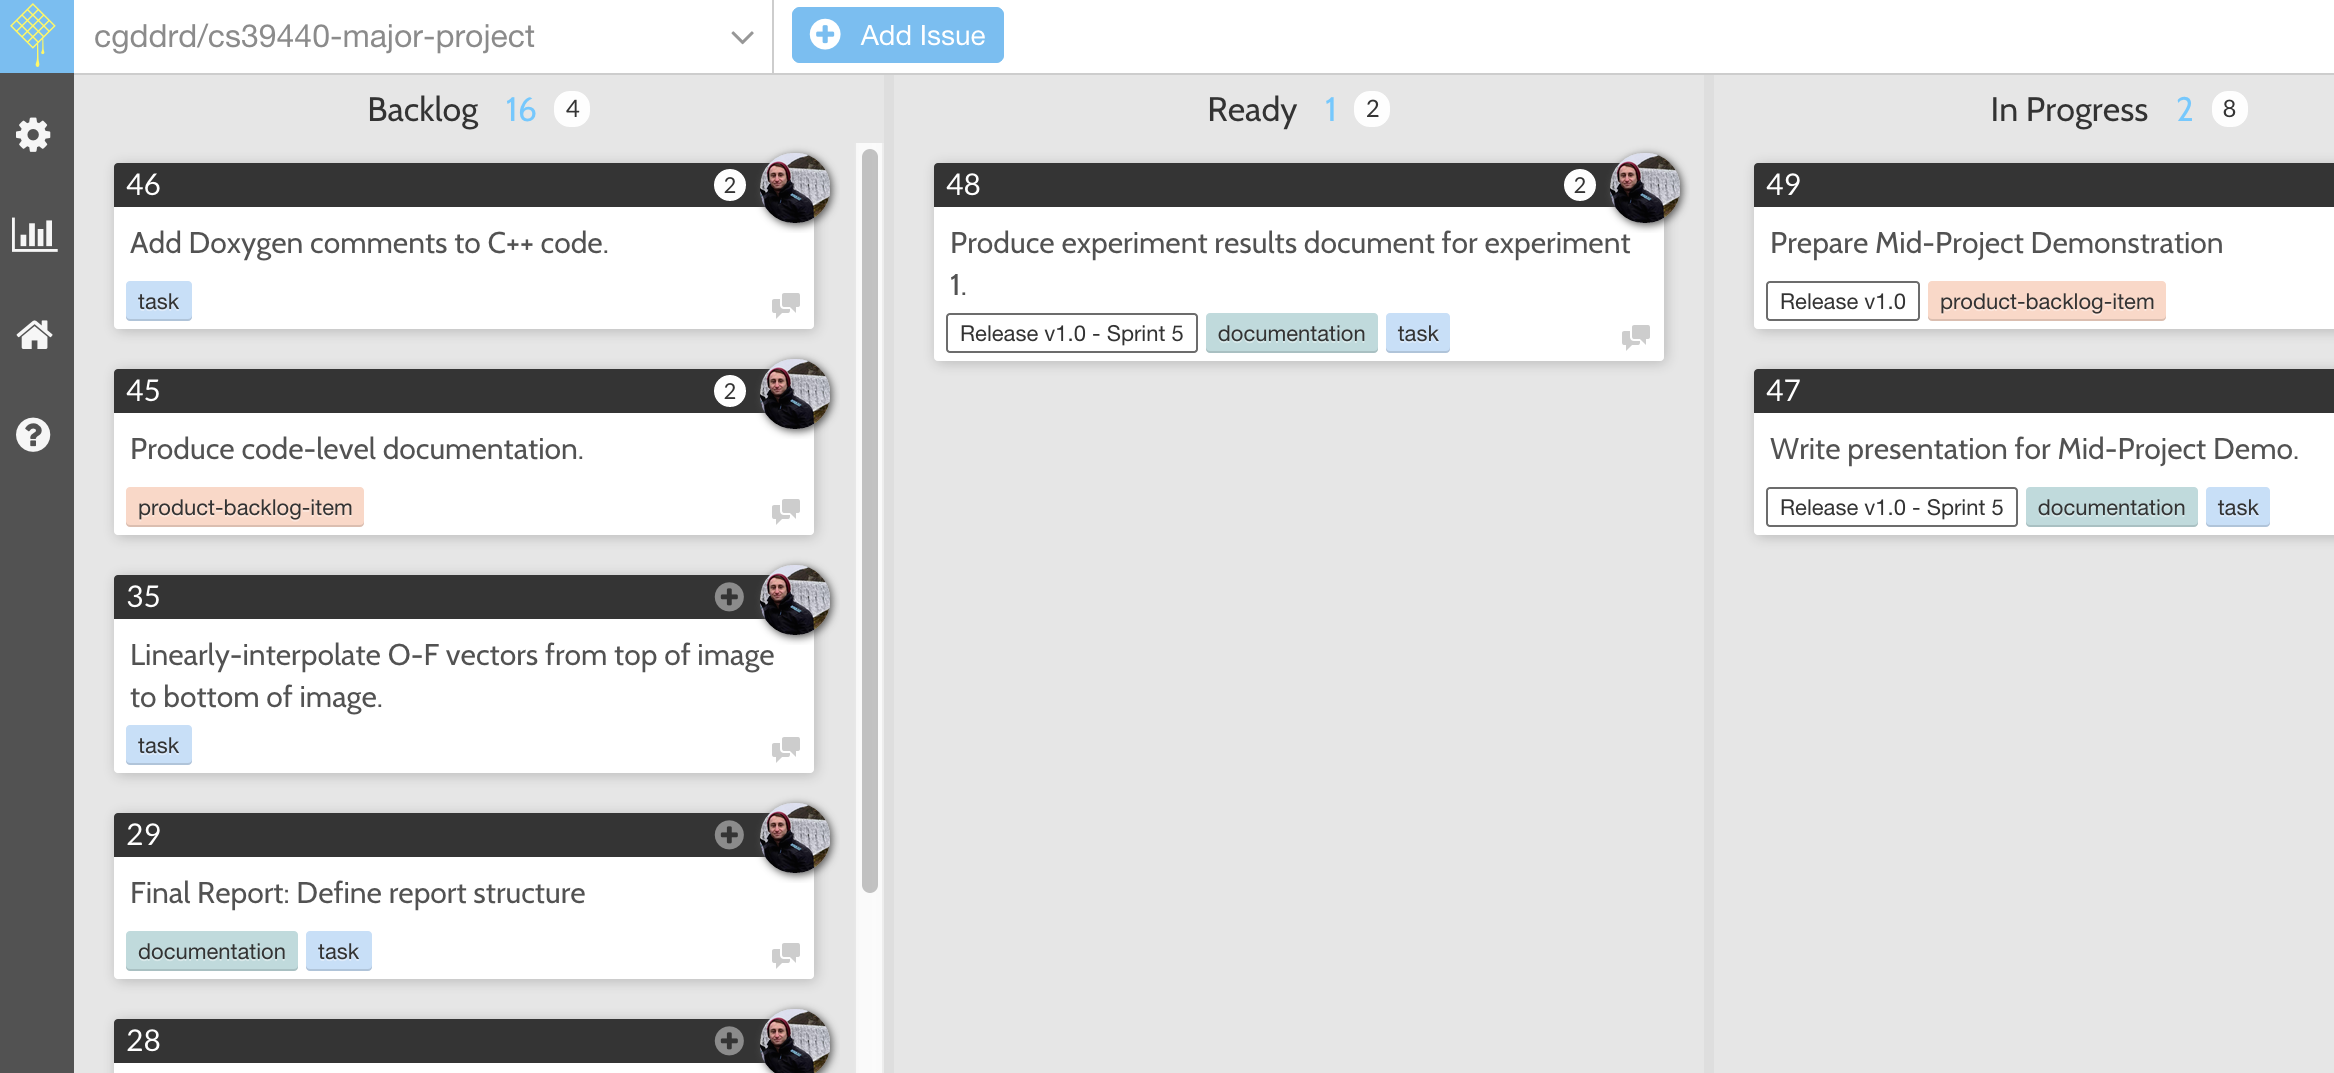
\includegraphics[scale=0.12]{waffle.png}
%\caption{Waffle.io KANBAN board interface to Github Issues.}
%\end{figure}
%
%\begin{figure}[ht!]
%\centering
%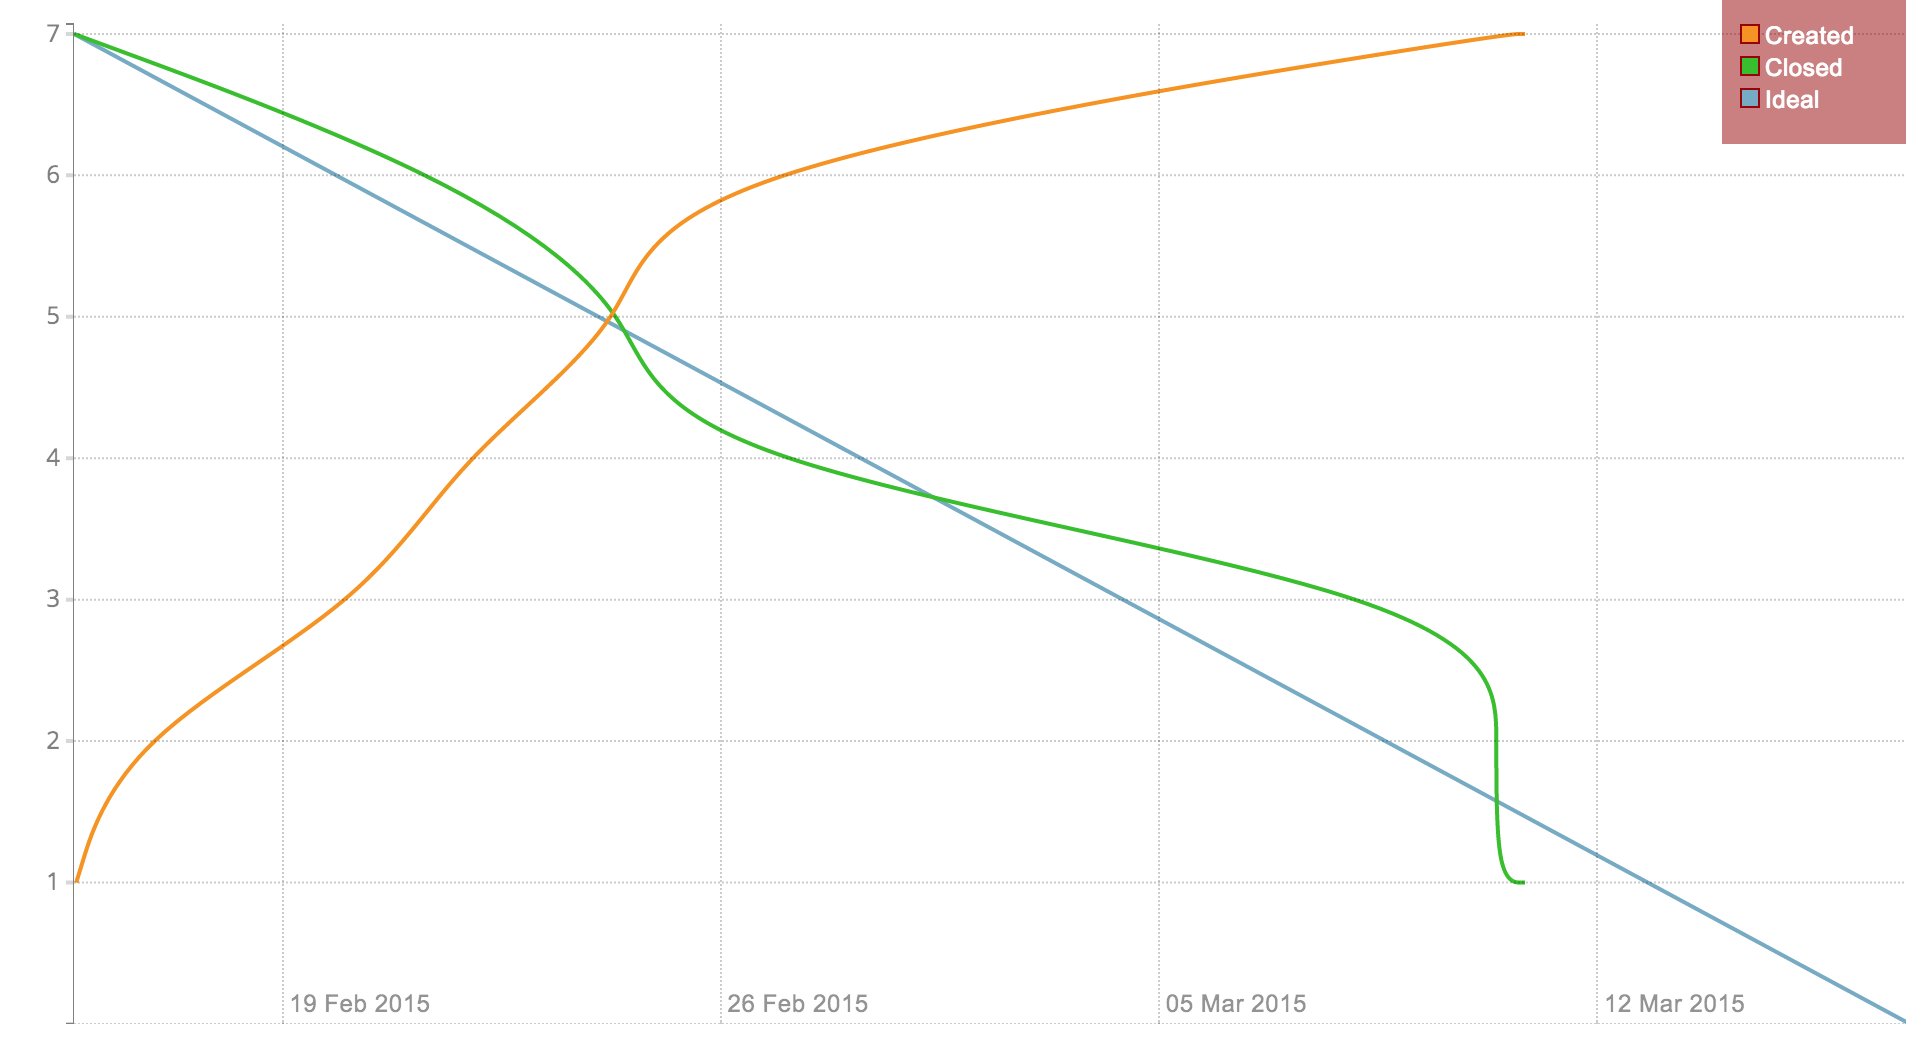
\includegraphics[scale=0.12]{burndown.png}
%\caption{Burndown chart for Release v1.0. \textbf{Courtesy:} \href{http://burndown.io}{http://burndown.io}}
%\end{figure}
%
%\end{frame}
%
%\begin{frame}{Next Steps}
%
%Plan is to move away from multiple small patches instead adopting a single, larger patch to represent a single row. \\ \vspace{0.5cm}
%
%Template patch will be scaled relative to its centre as the search moves down the image. This is to account for perspective distortion (\textbf{i.e.} objects becoming larger as they move closer to the camera).
%
%\begin{figure}[ht!]
%\centering
%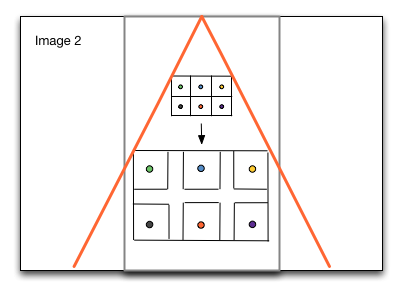
\includegraphics[scale=0.4]{scaling.png}
%\end{figure}
%	  
%\end{frame}

\plain{Questions? \\ \vspace{0.2cm} \footnotesize{\href{http://mmpblog.connorlukegoddard.com}{Project Blog} \\ \vspace{0.2cm} \footnotesize{Slide Design: Matthias Vogelgesang - (\href{https://github.com/matze/mtheme}{Github})}}}

\begin{frame}[fragile]
\frametitle{Bibliography}
\bibliographystyle{plain}
\nocite{maimone2007two, campbell, akshay, texas-cs, perveen}
\bibliography{mmp}
\end{frame}



\end{document}
